%!TEX root = ../Thesis.tex

\chapter{Realisierung der Fahrspurerkennung}
\label{cha:realisation}

In diesem Kapitel wird die Realisierung des Spurerkennungsalgorithmus thematisiert.
Es wird zuerst darauf eingegangen, wie die Trajektoriedaten im Algorithmus repräsentiert
und, vor der Clusteranalyse, vorverarbeitet werden.
Anschließend wird beschrieben, wie in den Trajektoriedatensätzen Cluster identifiziert werden,
welche den Verlauf von Fahrspuren beschreiben.
Den Schluss des Kapitels bildet die Vorstellung des Vorgehens zur Bestimmung der Spur-Geometrien.

\section{Repräsentation und Vorverarbeitung der Trajektoriedaten}
\label{cha:realisation_clustering}

Nachfolgend wird beschrieben, welche Repräsentation für die Trajektoriedaten in dieser Arbeit gewählt
wurde und welche Vorverarbeitungsschritte die Trajektorien vor der Clusteranalyse durchlaufen.

\subsection{Trajektorie-Repräsentation}

Die Ergebnisse der Fahrzeugverfolgung (siehe Abschnitt \ref{sec:position_extraction}) werden
in der Anwendung \textit{Vehicle-Tracker} in Form sogenannter \textit{TrackedObject}s gespeichert.
Ein solches Objekt repräsentiert eine zusammenhängende, nicht unterbrochene Verfolgung eines Fahrzeugs.
Wird eine Verfolgung, beispielsweise aufgrund einer Überdeckungen, unterbrochen, so existieren für ein
Kraftfahrzeug mehrere Objekte, welche sich nicht einander zuordnen lassen.
Die wichtigsten Informationen, die ein \textit{TrackedObject} beinhaltet, sind eine eindeutige ID,
die Frame-Positionen des Starts und Endes der Verfolgung und die Objekt-Klasse des Fahrzeugs. Es wird
zwischen den vier Klassen \textit{``Auto''}, \textit{``Lastwagen''}, \textit{``Transporter''}
und \textit{``Zweirad''} unterschieden.
Für jedes verfolgte Objekt können die zugehörigen Positions-, Geschwindigkeits-, Beschleunigungs-
und Größen-Informationen abgerufen werden. Diese werden für jedes Video-Frame, welches zwischen dem Start-
und End-Frame des Objektes liegt, bestimmt.

Da für die Ableitung von Fahrspuren aus Trajektorien lediglich die positionsbezogenen Eigenschaften
der Fahrzeuge relevant sind, werden Bewegungbahnen in dieser Arbeit nur über jene definiert.
Geschwindigkeit, Beschleunigung und Größe der Fahrzeuge werden in der Clusteranalyse nicht berücksichtigt.

Zur Erzeugung der Trajektorien werden die ``Front-Positionen'' der verfolgten Objekte verwendet. Diese markieren den
vordersten Punkt eines Fahrzeugs in einem bestimmten Video-Frame und befinden sich immer auf dessen Bounding-Box.
Idealerweise liegt die Front-Position auf der Stoßstange eines Fahrzeugs. In Abbildung \ref{fig:real1_tracked_object_front_position}
sind beispielhaft zwei verfolgte Objekte dargestellt. Die Front-Positionen werden durch die runden Markern angezeigt.

\begin{figure}[H]
    \centering
    \subfloat{{
        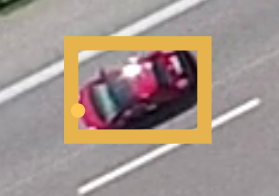
\includegraphics[align=c, width=0.23\linewidth]{resources/img/umsetzung/U1/CarInBB2}
    }}
    \qquad \qquad
    \subfloat{{
        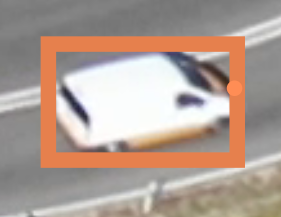
\includegraphics[align=c, width=0.23\linewidth]{resources/img/umsetzung/U1/CarInBB1}
    }}
    \caption{Erkannte Fahrzeuge und deren Front-Positionen}
    \label{fig:real1_tracked_object_front_position}
\end{figure}

Der Vorteil, welcher sich durch die Verwendung der Front-Positionen ergibt, ist, dass diese auch bei niedrigen
Aufnahmewinkeln nicht zu weit vom Mittelpunkt der Fahrspur, auf welchem sich das Fahrzeug befindet, entfernt liegen.
Dies ermöglicht eine bessere Bestimmung der Fahrspuren bei niedrigen Aufnahemwinkeln.

Abbildung \ref{fig:real_trajectory_classDia} zeigt den Aufbau einer Trajektorie im Modul \textit{Spurerkennung}.

\begin{figure}[H]
\centering
    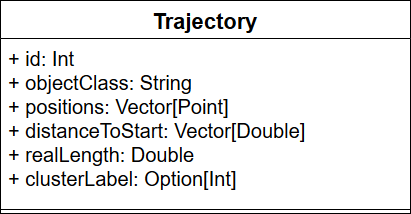
\includegraphics[width=0.35\linewidth]{resources/img/umsetzung/U1/Trajectory_ClassDia}
\caption{Aufbau Trajektorie-Klasse}
\label{fig:real_trajectory_classDia}
\end{figure}

Die Felder \textit{id} und \textit{objectClass} werden aus dem, der Trajektorie zugrundeliegenden, \textit{TrackedObject}
übernommen.
Die Positionen eines Fahrzeugs werden in Form von 2D Weltkoordinaten (siehe Abschnitt \ref{sec:position_extraction})
in \textit{positions} gespeichert und die Anzahl der Koordinaten zusätzlich in \textit{pointLength}.
Die Sequenz \textit{distToStart} enthält für jeden Punkt der Bewegungsbahn dessen Distanz zum Start der Trajektorie in Metern.
Die Werte ergeben sich aus Formel \ref{eq_real_distToStart}, wobei $p_n$ dem $n$-ten Punkt in der Trajektorie entspricht
und $dist$ der euklidschen Distanz zwischen zwei Punkten.

\begin{ceqn}
\begin{align}
\label{eq_real_distToStart}
    distToStart(p_n) =
    \begin{cases}
        0 & \text{if } n = 0 \\
        dist(p_n,\ p_{n-1}) + distToStart(p_{n-1}) & \text{otherwise}
    \end{cases}
\end{align}
\end{ceqn}

Aus \textit{distToStart} ergibt sich zudem die Gesamtlänge einer Trajektorie, welche extra gespeichert wird.
Das Feld \textit{clusterLabel} ordnet jede Trajektorie nach der Clusteranalyse einem bestimmten Cluster zu.
Zuvor enthält es keinen Wert.

Zur Untersuchung der Qualität der Fahrzeugtrajektorien ist es hilfreich diese zu visualisieren.
Abbildung \ref{fig:real_neckartor} b)
zeigt beispielsweise 1240 Trajektorien, welche aus einer Aufnahme des Stuttgarter Neckartors extrahiert wurden.
In Abbildung \ref{fig:real_neckartor} a) ist ein Video-Frame der entsprechenden Aufnahme zu sehen.

\begin{figure}[H]
    \centering
    \subfloat[]{{
        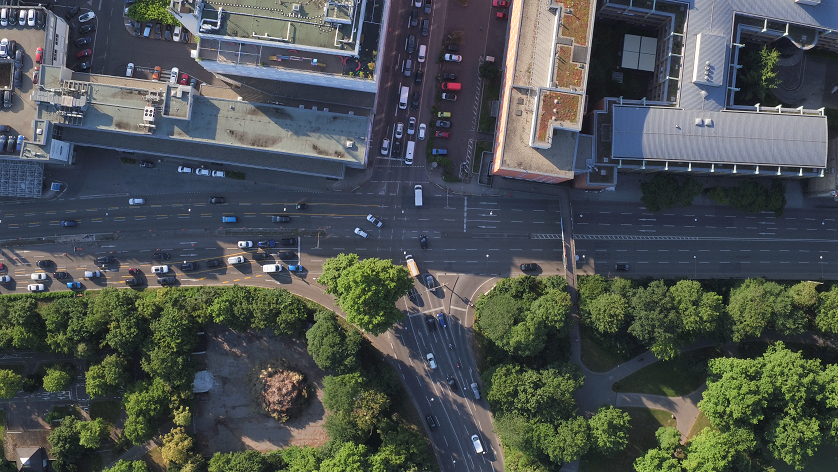
\includegraphics[align=c, width=0.5\linewidth]{resources/img/umsetzung/U1/Neckartor_Aufnahme}
    }}
    \subfloat[]{{
        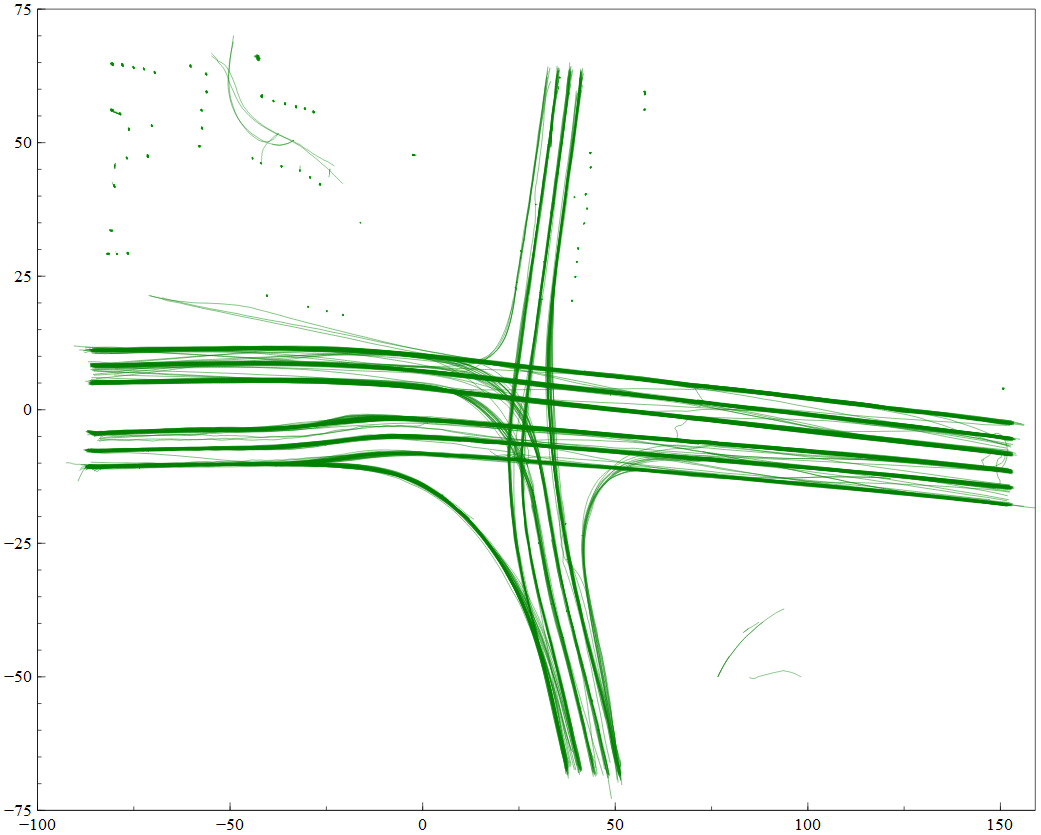
\includegraphics[align=c, width=0.42\linewidth]{resources/img/umsetzung/U1/Plot_RawTrajectories_Neckartor}
    }}
    \caption[Stuttgarter Neckartor und rekonstruierte Trajektorien]{Aufnahme Stuttgarter Neckartor a) und rekonstruierte Trajektorien b)}
    \label{fig:real_neckartor}
\end{figure}

In Abbildung \ref{fig:real_neckartor} b) sind die verschiedenen Bewegungsbahnen der Fahrzeuge für
den menschlichen Betrachter bereits klar erkennbar.
Es fallen allerdings auch die Trajektorien der stehenden oder sich auf Parkplätzen
bewegenden Autos im oberen Bereich der Aufnahme ins Auge. Diese dürfen nicht in die Clusteranalyse mit einbezogen werden,
da sie keine Bewegung auf einer Fahrbahn beschreiben.
Bei genauerer Untersuchung der Trajektorien zeigen sich weitere Probleme, welche das Clustering negativ
beeinflussen würden.
Zwei sind in Abbildung \ref{fig:real_defects_trajectories} dargestellt.
Teil a) zeigt, wie Fahrzeuge Punktwolken beim Stilstand vor Lichtsignalanlagen bilden.
Teil b) der Abbildung veranschaulicht, dass in bestimmten Bereichen sehr viele Trajektorie-Unterbrechungen
existieren.
In diesen Bereichen werden die Fahrbahnen üblicherweise von Bäumen, Brücken et cetera überlagert, wodurch
die Fahrzeugverfolgung unterbrochen wird (siehe Abschnitt \ref{sec:grund_challenges_reconstruction}).

\begin{figure}[H]
    \centering
    \subfloat[]{{
        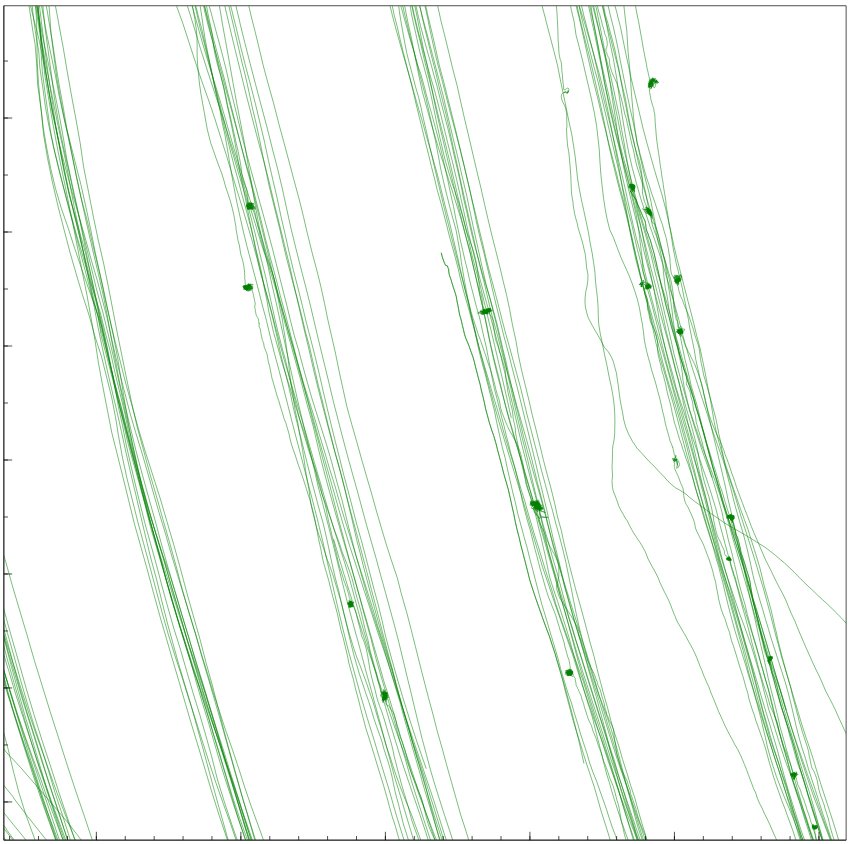
\includegraphics[align=c, width=0.28\linewidth]{resources/img/umsetzung/U1/trajectories_defect1}
    }}
    \qquad
    \subfloat[]{{
        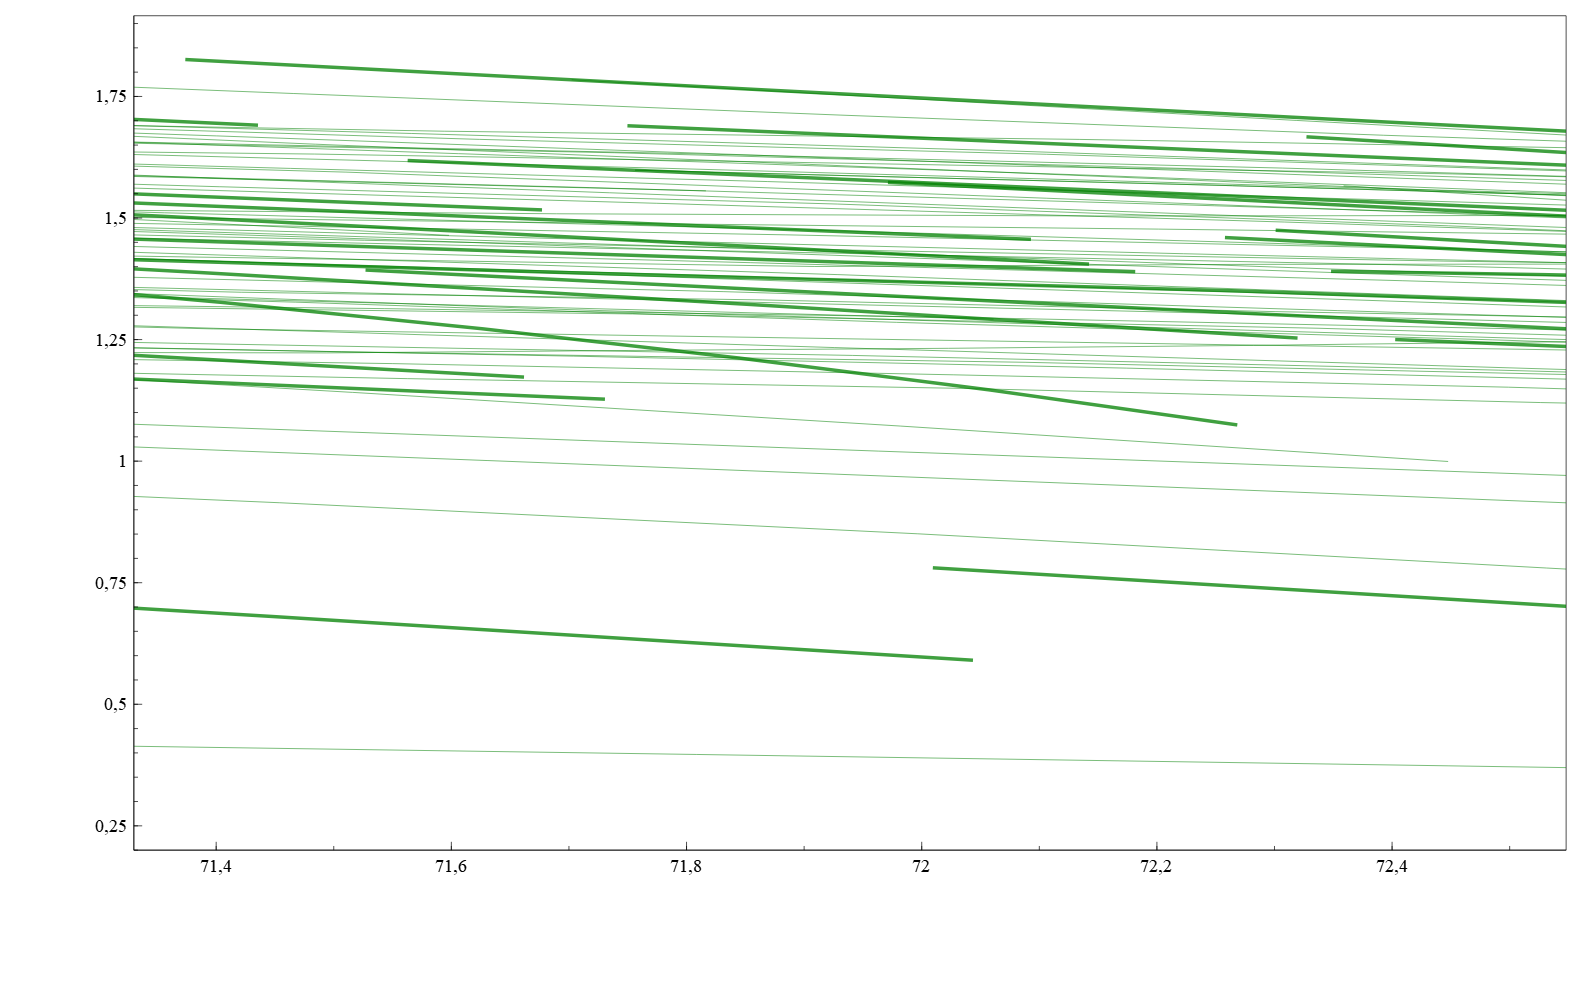
\includegraphics[align=c, width=0.37\linewidth]{resources/img/umsetzung/U1/trajectories_defect2}
    }}
    \caption[Beispiel Defekte in Trajektoriedaten]
            {Defekte in Trajektorien - Punktwolken vor Lichtsignalanlagen a), Unterbrechungen aufgrund von Fahrbahnverdeckung b)}
    \label{fig:real_defects_trajectories}
\end{figure}

Um von diesen und weiteren Effekten bei der Clusteranalyse nicht beeinflusst zu werden, durchlaufen die
``Roh-Trajektorien'' einen Vorverarbeitungsschritt. Dieser wird im nächsten Abschnitt beschrieben.

\subsection{Vorverarbeitung der Trajektorien}
\label{sec:realisation_preprocessing}

Primäres Ziel der Vorverarbeitung ist es, Ausreißer aus der
Trajektorie-Menge zu entfernen, welche das Ergebnis der Clusteranalyse negativ beeinflussen würden.
Die Qualität der Rohdaten hängt von der Qualität des verwendten Verfahrens zur Rekonstruktion von Fahrzeugtrajektorien
ab. Welche Probleme hierbei auftreten und wie sich diese auf die Trajektoriedaten auswirken, wurde bereits in
Abschnitt \ref{sec:grund_challenges_reconstruction} beschrieben.

Idealerweise sollen nach der Vorverarbeitung nur jene Trajektorien weiterverarbeitet werden,
welche eine ununterbrochene Bewegung eines Fahrzeugs auf einem bestimmten Straßenabschnitt beschreiben.
Anhand dieser Trajektorien kann anschließend die Geometrie der realen Fahrspuren ermittelt werden.

In folgender Auflistung sind die drei wichtigsten Vorverarbeitungsschritte aufgeführt:

\begin{enumerate}
    \item Resampling von Trajektorien auf minimale Punktdistanz,
    \item Entfernung zu kurzer Trajektorien und
    \item Entfernung unterbrochener Trajektorien
\end{enumerate}

Die einzelnen Schritte und ihre Hintergründe werden anschließend noch genauer erläutert.

\subsubsection{Resampling von Trajektorien auf minimale Punktdistanz}
Der erste Vorverarbeitungsschritt reduziert die Anzahl der Koordinaten, welche eine Bewegungsbahn beschreiben, erheblich.
Es gehen dabei jedoch keine wichtigen Informationen verloren.
Insbesondere dann, wenn sich Fahrzeuge mit niedrigen
Geschwindigkeiten bewegen oder teilweise vor Ampeln et cetera halten, bestehen die Roh-Trajektorien aus sehr vielen
Punkten, welche beinahe identische Positionsinformationen darstellen, das heist nur sehr geringe
Abstände voneinander haben. Für die Beschreibung einer Bewegungsbahn ist diese hohe Punktdichte nicht notwendig
und sogar kontraproduktiv, da sie die Performance der nachfolgenden Schritte negativ beeinflusst.

Aus diesen Gründen werden im ersten Vorverarbeitungsschritt Trajektorien \textit{resampled}, so dass die Distanz
aufeinanderfolgender Punkte mindestens $1.5\ m$ beträgt.
Der hierzu verwendete Algorithmus ist in Listing \ref{lst:pseudo_resampling} dargestellt.
Er verwirft alle aufeinanderfolgende Punkte, welche von einem Referenzpunkt weniger als den geforderten Abstand haben.
\begin{lstlisting}[caption=Pseudocode Trajektorie Resampling, language=Pseudo, label=lst:pseudo_resampling]
algorithm resampleTrajectory:
  input:  lastRefPoint, newTrajPoints, oldTrajPoints
  output: resampled trajectory points

  while oldTrajPoints is not empty do:
    nextPoint := Head(oldTrajPoints)
    remPoints := Tail(oldTrajPoints)

    if dist(lastRefPoint, nextPoint) < 1.5:
      resampleTrajectory(lastRefPoint, newTrajPoints, remPoints)
    else:
      resampleTrajectory(nextPoint, newTrajPoint ++ nextPoint, remPoints)
    end
  end

  return newTrajPoints
\end{lstlisting}

Nach Anwendung des Algorithmus ist im Fall der Neckartor Aufnahme die durchschnittliche Punktlänge
der Trajektorien von 1094 Koordinaten auf 65 gesunken. Die realen Längen der Bewegungsbahnen bleiben
hingegen nahezu identisch. Die Punktwolken, welche stehende Fahrzeuge erzeugen, werden mittels dieses
Schritts ebenfalls entfernt (siehe Abb. \ref{fig:real_result_2nd_Prepro} b)).

\subsubsection{Entfernung von zu kurzen Trajektorien}
Der zweite Verarbeitungsschritt entfernt viele Trajektorien von beispielsweise stehenden Fahrzeugen
oder kurz auftretenden Tracking-Fehlern.
Hierzu wird die Länge aller Trajektorien überprüft und jene entfernt, welche
unter einem bestimmten Grenzwert liegen. Die hierzu verwendete boolesche Überprüfung ist in Gleichung
\ref{eq_isShortTrajectory} gegeben.
Als Standardwert für $minLength$ wurde experimentell $20m$ bestimmt, da dies für alle
Testaufnahmen gute Ergebnisse lieferte. Bei Bedarf kann der Anwender den Parameter beim Start des Spurerkennungs-Jobs
in der Oberfläche anpassen.

\begin{ceqn}
\begin{align}
\label{eq_isShortTrajectory}
    isShortTrajectory(t) =
    \begin{cases}
        1 & \text{if } t.realLength < minLength \\
        0 & \text{otherwise}
    \end{cases}
\end{align}
\end{ceqn}

Das Ergebnis der ersten beiden Vorverarbeitungsschritte ist in Abbildung \ref{fig:real_result_2nd_Prepro} dargestellt.
Die Trajektorien stehender Fahrzeuge, sowie die Punktwolken vor Lichtsignalanlagen und weitere Defekte aufgrund
kleiner Tracking-Fehler wurden entfernt.

\begin{figure}[H]
    \centering
    \subfloat[]{{
        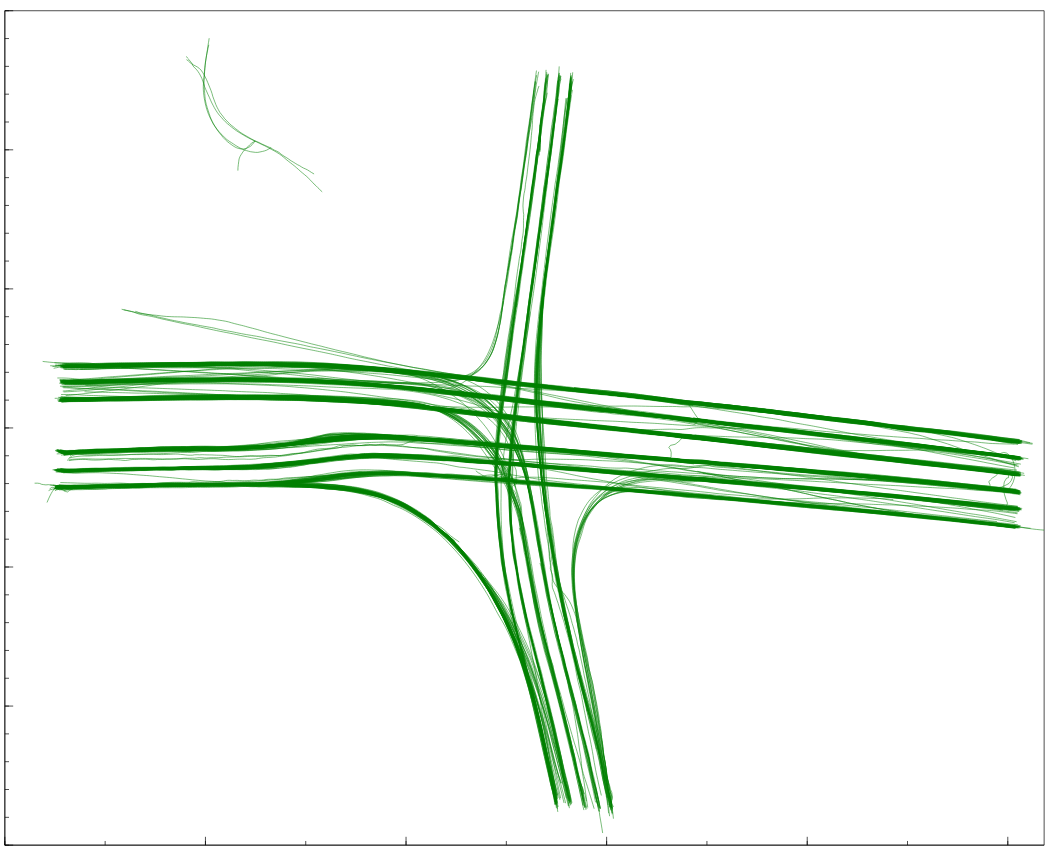
\includegraphics[align=c, width=0.4\linewidth]{resources/img/umsetzung/U1/trajectories_resampledFiltered}
    }}
    \qquad \qquad
    \subfloat[]{{
        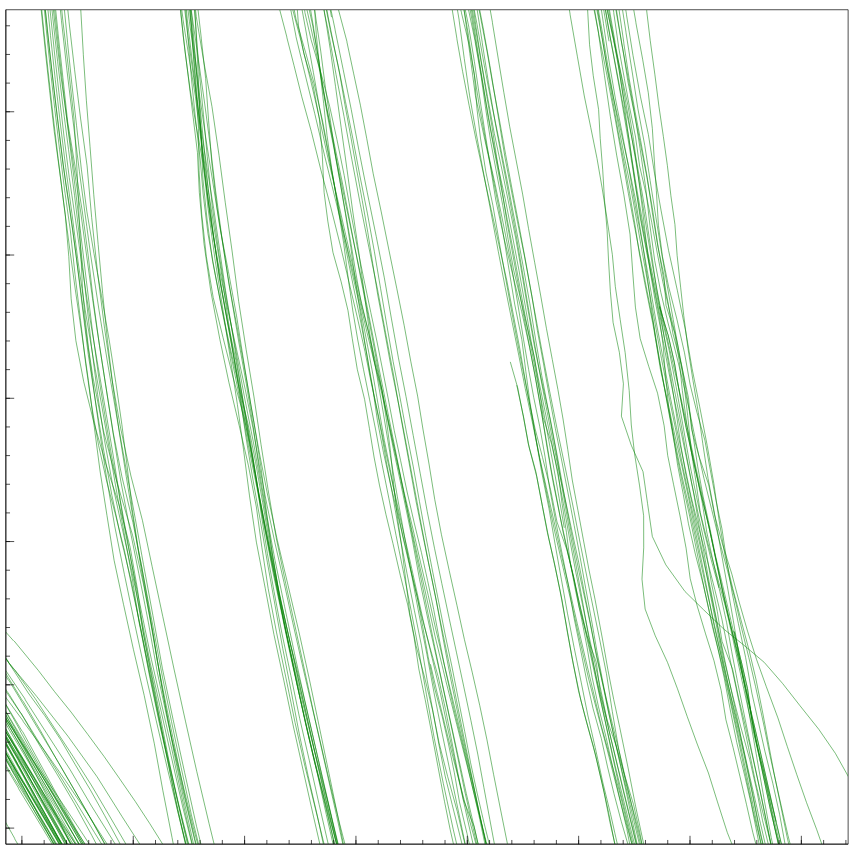
\includegraphics[align=c, width=0.33\linewidth]{resources/img/umsetzung/U1/trajectories_resampled_cleared}
    }}
    \caption[Ergebnisse der zwei ersten Vorverarbeitungsschritte]
            {Ergebnisse der zwei ersten Vorverarbeitungsschritte - Übersicht (keine stehenden Trajektorien) a), Detailansicht (keine Punktwolken) b)}
    \label{fig:real_result_2nd_Prepro}
\end{figure}


\subsubsection{Entfernung unterbrochener Trajektorien}
\label{sec:real1_remove_broken_trajectories}

Nachdem durch die ersten beiden Vorverarbeitungsschritte bereits viele Defekte entfernt wurden,
müssen nun noch unterbrochene Verfolgungen ausgefiltert werden, da diese das Ergebnis der Clusteranalyse
negativ beeinflussen.

Der erste verwendete Ansatz zur Entfernung von unterbrochenen Trajektorien beruhte auf der Annahme,
dass komplette Trajektorien immer im Bereich der Szenenränder beginnen und enden. Daher wurden alle Trajektorien,
welche diese Bedingung nicht erfüllen, entfernt. Es ist jedoch auch möglich, dass ununterbrochene Trajektorien
in der Mitte einer Aufnahme beginnen, wenn die verfolgten Fahrzeuge in diesem Bereich beispielsweise
aus einem Tunnel hervorkommen. Unter Anwendung des obigen Ansatzes würden diese Trajektorien
fälschlichweise entfernt. Daher wurde ein alternatives Vorgehen implementiert.

Das im Algorithmus eingesetzte Verfahren basiert auf einer anderen Definition von unterbrochenen
Trajektorien: Bewegungsbahnen gelten dann als unterbrochen, wenn sich auf Höhe ihrer Starts
oder Enden mehrere Trajektorien befinden, welche auf der entsprechenden Höhe nicht starten oder enden.
Ist dies der Fall, dann gilt die untersuchte Bewegungsbahn als unterbrochen. Die angrenzenden Trajektorien
sind potenziell vollständig, das heißt ununterbrochen.
Abbildung \ref{fig:real_completeTrajectory} veranschaulicht dieses Konzept.

\begin{figure}[H]
\centering
    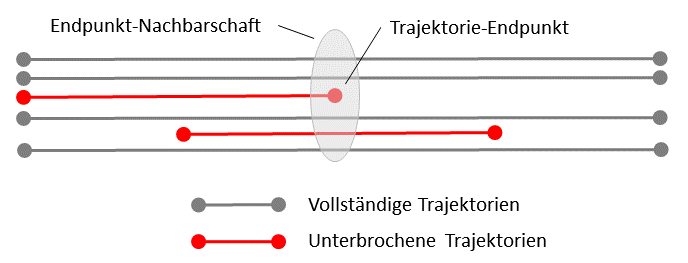
\includegraphics[width=0.6\linewidth]{resources/img/umsetzung/U1/complete_trajectories_concept}
\caption{Konzept Identifikation von unterbrochenen Trajektorien}
\label{fig:real_completeTrajectory}
\end{figure}

Der Algorithmus zur Entfernung unterbrochener Trajektorien nutzt die oben gegebene Definition.
Er untersucht von allen Trajektorien die Nachbarschaften der Start- und Endpunkte. Befinden sich in
den Nachbarschaften mindestens 25\% der Punkte nicht am Rand der entsprechenden Trajektorien, so wird
die untersuchte Bewegungsbahn als unterbrochen gewertet und entfernt.
Dieses Vorgehen beruht auf der Annahme, dass für eine Fahrspur neben unterbrochenen auch
ununterbrochene Trajektorien vorliegen, welche eine vollständige Bewegung auf der Spur beschreiben,
was üblicherweise der Fall ist.

Nach Ausführung dieses Filter-Schrittes, besteht die Menge der übrigen Trajektorien nurnoch
aus ununterbrochenen Bewegungsbahnen, welche Bewegungen von Fahrzeugen auf einem bestimmten
Straßenabschnitt beschreiben.

\section{Clusteranalyse der Trajektorien}
\label{sec:realisation_clustering}

Nachdem im vorherigen Abschnitt beschrieben wurde, wie die Roh-Trajektorien vorverarbeitet
werden, folgt nun eine Erläuterung zweier Verfahren zur Clusteranalyse von Trajektorien, deren Einsatz
im Rahmen der Arbeit genauer untersucht wurde.

\subsection{Ansatz Spectral-Clustering und modifizierte Hausdorff-Distanz}
\label{sec:real_ansatz_spec_modHD}

Als erster Ansatz für die Clusteranalyse wurde das von \cite[]{Atev2010} vorgestellte Verfahren untersucht.
Es wurde gewählt, da es sowohl in der Arbeit von Atev et al. selbst, wie auch in \cite[]{Morris2009}, gute Ergebnisse
bei der Clusteranalyse lieferte.
Das Verfahren nutzt die in \cite[]{Atev2006} vorgestellte modifizierte Hausdorff-Distanz und den
Spectral-Clustering-Algorithmus. Die Grundlagen des Distanzmaßes wurden bereits in Abschnitt
\ref{sec:atev_et_al} beschrieben. Nachfolgend wird noch etwas genauer vorgestellt, wie die
modifizierte Hausdorff-Distanz berechnet wird. Anschließend
wird auf den eingesetzten Clusteralgorithmus und die erzielten Ergebnisse eingegangen.

\subsubsection{Das Verfahren}

Grundlegend war die modifizierte Hausdorff-Distanz nach Atev et al., wie in Gleichung \ref{eq_modHausdorff}
bereits definiert, gegeben als:

\begin{ceqn}
\begin{align*}
    h_{\alpha, N, C}(P, Q) = \overset{\alpha}{\underset{p \in P}{ord}}\ \Big\{ \underset{q \in N_Q(C_{P,Q}(p))}{min} d(p, q) \Big\}
\end{align*}
\end{ceqn}

Um die Distanz zwischen zwei Trajektorien $P$ und $Q$ zu bestimmen, müssen zuerst die minimalen Distanzen
zwischen allen Punkten $p \in P$ und deren Nachbarschaften $N_Q(C_{P,Q}(p))$ in $Q$ bestimmt werden.
Eine Nachbarschaft in $Q$ um den Punkt $q_0$ ist in Abhängigkeit des Parameters $w$ definiert als:

\begin{ceqn}
\begin{align}
    N_Q(q_0) = \{ q \in Q |\ |\pi_Q(q_0) - \pi_Q(q)| \le w/2 \}
\end{align}
\end{ceqn}

$\pi_Q(q)$ entspricht hierbei der relativen Position von $q$ in $Q$, welche in Gleichung \ref{eq_atev_relPos} definiert ist.
$|Q_j|$ steht für die Länge einer Trajektorie bis zum Punkt $j$ und $|Q|$ für die Gesamtlänge einer Bewegungsbahn.
Diese Längeninformationen sind beide in der verwendeten Trajektorie-Definition aus Abbildung
\ref{fig:real_trajectory_classDia} enthalten.

\begin{ceqn}
\begin{align}
\label{eq_atev_relPos}
    \pi_Q(q_j) = \frac{|Q_j|}{|Q|}
\end{align}
\end{ceqn}

Die Nachbarschaften werden um den Referenzpunkt $q \in Q$ gebildet, welcher die selbe relative Position
in $Q$ besitzt wie $p$ in $P$. Der Index dieses Punktes ergibt sich aus dem Mapping $C_{P,Q}$ wie folgt:

\begin{ceqn}
\begin{align}
\label{eq_atev_findPointAtRelPow}
    C_{P,Q}(p) = arg\ \underset{q \in Q}{min}\ |\pi_P(p) - \pi_Q(q)|
\end{align}
\end{ceqn}

Zur Berechnung der Distanzen $d(p,q)$ zwischen $p$ und allen Punkte $q \in N_Q(C_{P,Q}(p))$, wird die euklidsche
Distanz verwendet. Wurden auf diese Weise alle minimalen Distanzen zwischen Punkten und ihren Nachbarschaften in
der Vergleichs-Trajektorie bestimmt, so wird aus ihnen der finale Distanzwert bestimmt. Der Operator
$ord_{p \in P}^{\alpha}$ wählt hierfür jene Distanz, welche größer ist als $\alpha$-Prozent aller Werte.
Mit Hilfe dieses Distanzmaßes wird eine Distanz-Matrix $D$ konstruiert, welche die Distanzen
aller Trajektorie-Kombinationen speichert.

Um die modifizierte Hausdorff Distanz im Spectral-Clustering Verfahren einsetzten zu können, muss ein
zusätzliches Affinitätsmaß verwendet werden.
Dieses definieren Atev et al. als:

\begin{ceqn}
\begin{align}
    k(P,Q) = exp (- \frac{h_{\alpha, N, C}(P,Q)\ h_{\alpha, N, C}(Q,P)}{2 \sigma(P) \sigma(Q)})
\end{align}
\end{ceqn}

$\sigma(P)$ und $\sigma(Q)$ entsprechen hier Schätzungen für die Streuung der Distanzwerte einer Trajektorie
zu allen anderen Trajektorien. Sie ergeben sich aus der Distanz-Matrix $D$.

Der in dieser Arbeit und von Atev et al. verwendete Spectral-Clusteralgorithmus folgt grundsätzlich
der Standard-Definition von \cite[]{Ng2002}.
Für eine feste Clusteranzahl $k$ kann er wie folgt zusammengefasst werden:

\begin{enumerate}
    \item Erstellen einer Affinitätsmatrix $A \in \mathbb{R}^{n \times n}$ basierend auf dem Affinitätsmaß, wobei $A_{ii} = 0$
    \item Definieren einer Diagonalenmatrix $D$, deren Elemente an der Stelle $(i,i)$ der Summe der $i$-ten
            Zeile von $A$ entsprechen. Basierend auf $D$ wird die Matrix $L = D^{-1/2} AD^{-1/2}$ erstellt.
    \item Durchführen einer Eigenwert Dekomposition auf $L$, um die $k$ größten Eigenvektoren
            $\{x_1, x_2, ..., x_k\}$ zu finden.
    \item Erstellen einer Matrix $X = [x_1, x_2,..., x_k]$ durch spaltenweises Zusammenführen der Eigenvektoren und
            Normalisierung der Zeilen auf die Länge 1.
    \item Gruppierung der Zeilen von Matrix $X$ in $k$-Cluster unter Zuhilfenahme von k-Means et cetera.
            Jede Zeile wird als Datenpunkt interpretiert.
\end{enumerate}

Ein großer Nachteil des Spectral-Clustering-Ansatzes ist es, dass bei seiner Verwendung üblicherweise die Clusteranzahl $k$
bereits im vorraus bekannt und angegeben sein muss. Aus diesem Grund verwenden Atev et al. ein Schätzmaß für
$k$, welches darauf abzielt, die Verzerrung des in Schritt 5) eingesetzten k-Means Algorithmus zu minimieren.
Hierzu wird die k-Means Clusteranalyse mit mehreren $k$'s zwischen den Grenzen $kMin$ und $kMax$ durchgeführt
und anschließend jeweils ein Verzerrungs-Maß $\rho_k$ berechnet, welches angibt, wie gut die gefundenen Centroids
die Datenpunkte beschreiben. Für $k$ wird daher jener Wert gewählt, welcher das
kleineste $\rho_k$ erzeugt. Diese Methode zur Schätzung der Clusteranzahl wurde auch in der vorliegenden
Arbeit angewandt.
Die auf diese Weise mithilfe des Verfahrens von Atev et al. identifizierten Cluster-Sets sind partitioniert,
exklusiv und komplett (siehe Abschnitt \ref{sec:grund_property_cluster_sets}).

\subsubsection{Auswertung des Verfahrens}

Nachdem das Verfahren, wie in \cite[]{Atev2006} und \cite[]{Ng2002} beschrieben, implementiert wurde,
wurde eine Evaluation durchgeführt. Die Clustering-Performance des Ansatzes
wurde hierzu initial anhand von zwei Trajektoriedatensätzen untersucht.

Die Ergebnisse der Clusteranalyse für den einfacheren Datensatz sind in Abbildung \ref{fig:real_results_atev1}
dargestellt. An diesem Beispiel lassen sich die Probleme bereits identifizieren.
Für die Analyse wurden die Parameter $\alpha = 0.85$ und $w = 1.0$ verwendet.
Zur Bestimmung von $\sigma$ kamen die Grenzwerte $stdMin = 0.5$ und $stdMax = 10.0$ zum Einsatz.
Diese haben sich in unterschiedlichen Versuchen als am besten geeignet erwiesen.
Trotzdem ist in Abbildung \ref{fig:real_results_atev1} a) zu erkennen, dass nicht alle Fahrspuren einem
extra Cluster zugewiesen wurden.

\begin{figure}[H]
    \centering
    \subfloat[mit Schätzung Clusteranzahl]{{
        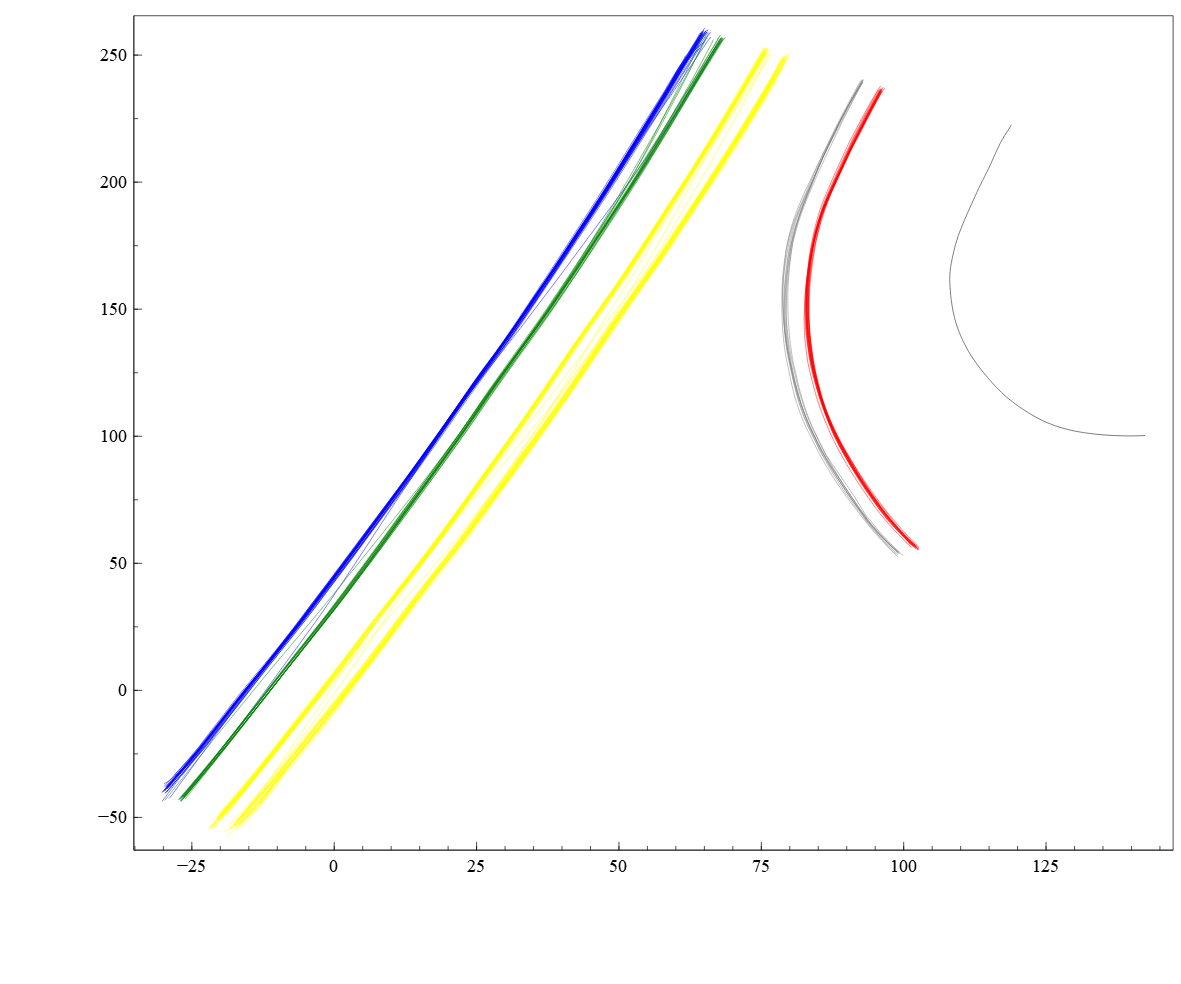
\includegraphics[align=c, width=0.4\linewidth]{resources/img/umsetzung/U1/atev_results/entennest_k_est}
    }}
    \qquad \qquad
    \subfloat[mit fester Clusteranzahl]{{
        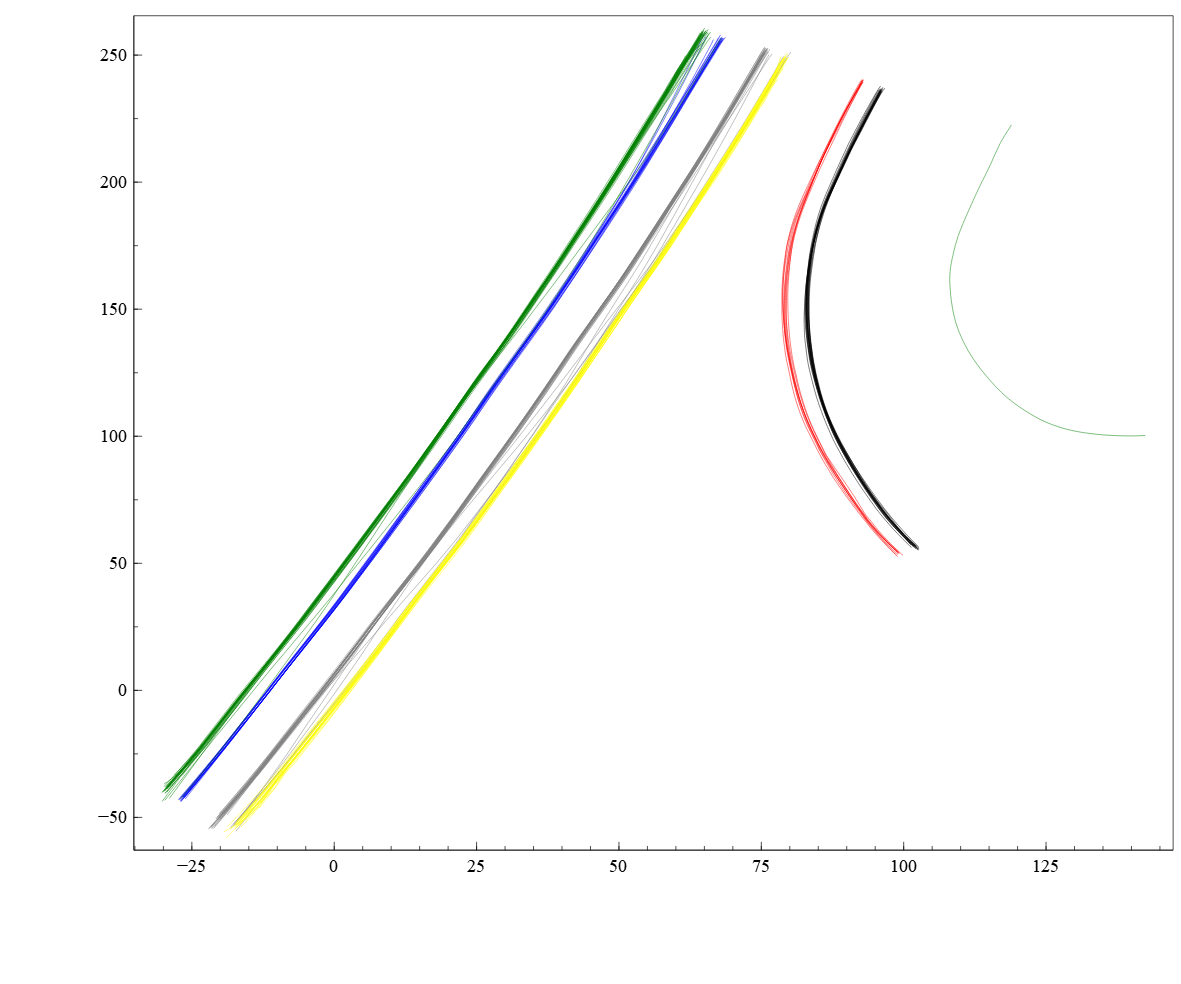
\includegraphics[align=c, width=0.4\linewidth]{resources/img/umsetzung/U1/atev_results/entennest_k6}
    }}
    \caption[Ergebnisse Clusteranalyse Ansatz Atev et al.]
            {Ergebnisse Clusteranalyse Ansatz Atev et al. - fehlerhaftes Clusterergebnis in a), gewünschtes Ergebnis in b)}
    \label{fig:real_results_atev1}
\end{figure}

Ein erstes Problem des Verfahrens sind die vielen Parameter und Grenzwerte, welche vom Anwender bestimmt werden müssen und
nicht alle intuitiv verständlich sind.
Neben den oben aufgeführten Parametern, gibt es noch weitere, welche bei der Bestimmung der Clusteranzahl und der
Berechnung des Affinitätsmaßes zum Einsatz kommen.
Eine Optimierung der Parameter und somit der erzielten Ergebnisse wäre sicherlich möglich gewesen,
hierauf wurde aber aufgrund anderer existierender Schwierigkeiten verzichtet.

Problematisch ist das Vorgehen auch, da der Spectral-Clusteralgorithmus nicht mit Ausreißern umgehen kann,
welche trotz der Vorverarbeitung der Trajektorien immer noch in geringer Anzahl in den Datensätzen vorhanden seien können.
In Abbildung \ref{fig:real_results_atev1} a) und b) ist beispielsweise die einzelne Fahrspur im oberen, rechten Bereich
einem Spur-Cluster zugeordnet, was nicht korrekt ist.
Diese falsche Zuordnung der Ausreißer, würde die Bestimmung der Spur-Geometrien im nächsten Schritt des
Algorithmus aus Abschnitt \ref{fig:concept_laneDetection_activity} erschweren.

Die schlechten Clustering-Ergebnisse des Ansatzes sind primär Folge der nicht zuverlässig funktionierenden Schätzung
der Clusteranzahl $k$. Im Fall des Datensatzes aus Abbildung \ref{fig:real_results_atev1}, wird $k = 5$
statt korrekterweise $k = 6$ geschätzt. Hieraus ergibt sich, dass in Abbildung \ref{fig:real_results_atev1} a)
zwischen zwei Fahrspuren nicht richtig unterschieden wird. In Teil b) wurde die Clusteranzahl händisch spezifiziert,
was in einer korrekten Gruppierung der Fahrspuren resultierte.

Ausschlaggenend dafür, dass der Ansatz von Atev et al. nicht weiter verfolgt und optimiert wurde, war schlussendlich
jedoch die Performance der Clusteranalyse. Für den Trajektoriedatensatz aus Abbildung \ref{fig:real_results_atev1},
welcher nach der Vorverarbeitung nur 132 Bewegungsbahnen beinhaltet, benötigt die Clusteranalyse bereits über
90 Sekunden. Für einen Datensatz mit über 400 Trajektorien, beträgt die Verarbeitungsdauer über 8 Minuten.
Die schlechte Performance lässt sich auf das aufwendige Distanz- und Affinitätsmaß, aber auch auf die mehrfache
Durchführung des k-Means Algorithmus zurückführen.

Aufgrund der oben angeführten Problematiken, welche auch bei der Anwendung des Verfahrens auf andere Datensätze auftraten,
wurde entschieden, dass der Ansatz nicht weiter verfolgt werden soll.
Es wurde ein Ansatz gesucht, welcher mit den beschriebenen Herausforderungen besser umgehen kann.

\subsection{Ansatz DBSCAN und LCSS}
\label{sec:real_ansatz_dbscan_lcss}

Nachdem das in Abschnitt \ref{sec:real_ansatz_spec_modHD} beschriebene Verfahren in
den Untersuchungen schlechte Ergebnisse lieferte, wurde nach neuen Ansätze gesucht.
Kriterien für diese waren primär, dass sie mit Ausreißern sinnvoll umgehen können, weniger Parametrisierung
benötigen beziehungsweise diese intuitiver ist, und sie eine bessere Performance besitzen.
Aufgrund dieser Anforderungen wurde untersucht, inwiefern sich der DBSCAN-Clusteralgorithmus
in Kombination mit dem LCSS-Distanzmaß für die Clusteranalyse von Trajektoriedaten eignet.

Vorteil des dichte-basierten DBSCAN-Algorithmus, dessen Funktionsweise bereits in Abschnitt
\ref{sec:grund_density_clustering} erläutert wurde, ist, dass er Ausreißer erkennt und die Anzahl der
Zielcluster selbstständig bestimmen kann.
Die auf diese Weise identifizierten Cluster-Sets sind also, ebenso wie bei Atev et al., partitioniert und exklusiv,
sind aber außerdem partielle (siehe Abschnitt \ref{sec:grund_property_cluster_sets}).
Das LCSS Distanzmaß, grundlegend in Abschnitt \ref{sec:lcss_distance}
beschrieben, ähnelt der modifizierten Hausdorff-Distanz, lässt sich allerdings performanter implementieren
und besitzt eine intuitivere Parametrisierung. Es lieferte in den Arbeiten \cite[]{Morris2011} und
\cite[]{Chen2014} gute Clustering-Ergebnisse.

\subsubsection{Das Verfahren}

Die Grundgleichung des LCSS Distanzmaßes wurde, basierend auf \cite[]{Vlachos2002}, bereits in Gleichung
\ref{eq_lcss} definiert und ist nachfolgend nochmals dargestellt.

\begin{ceqn}
\begin{align*}
    LCSS_{\epsilon, \delta}(t_1, t_2) =
    \begin{cases}
        0 & \text{if } t_1 \text{ or } t_2 \in \emptyset \\
        1 + LCSS_{\epsilon, \delta}(t_1', t_2') & \text{if } dist(t_1(n), t_2(m)) < \epsilon \\
        & \land\ |n - m| \leq \delta \\
        max(LCSS_{\epsilon, \delta}(t_1', t_2), LCSS_{\epsilon, \delta}(t_1, t_2')) & \text{otherwise}
    \end{cases}
\end{align*}
\end{ceqn}

Mit ihrer Hilfe lässt sich bestimmen, wie groß die längste, übereinstimmende Subsequenz zweier Trajektorien
$t_1$ und $t_2$ ist. Damit Punkte zweier Trajektorien als übereinstimmend gewertet werden, dürfen sie
höchstens die Distanz $\epsilon$ zueinander haben und ihre Position in den Bewegungsbahnen sich höchstens um $\delta$
unterscheiden.
Wenn das Zählmaß, wie oben dargestellt, rekursiv implementiert wird, liegt die Zeitkomplexität des Algorithmus
bei $O(2^n)$, was für den Vergleich einer größeren Anzahl von Trajektorien nicht geeignet ist. Die Performance
kann auf $O(m\ n)$ verbessert werden, indem das Maß mit Hilfe von dynamischer Programmierung und \textit{Memoization}
umgesetzt wird. Der sich so ergebende Algorithmus ist in Listing \ref{lst:pseudo_LCSS} aufgeführt.
\begin{lstlisting}[caption=Pseudocode LCSS Bestimmung, language=Pseudo, label=lst:pseudo_LCSS]
algorithm LCSS:
  input:  trajectory: t1, trajectory: t2, epsilon, deltaFac
  output: LCSS distance between t1 and t2

  t1Len := point-length t1
  t2Len := point-length t2
  delta := deltaFac * min(t1Len, t2Len)
  LCS := 2D array with dims. (t1Len+1, t2Len+1)

  for i <- 1 to t1Len do:
    for j <- 1 to l2Len do:
      if dist(t1(i-1), t2(j-1)) < epsilon && |i-j| < delta then:
        LCS(i)(j) = LCS(i-1)(j-1) + 1
      else
        LCS(i)(j) = max(LCS(i-1)(j), LCS(i)(j-1))
      end
    end
  end

  return LCS(t1Len)(t2Len)
\end{lstlisting}

Der Parameter $\delta$ wurde in dieser Implementierung nicht, wie meist üblich, fest definiert, sondern er ergibt sich als
ein Teil der Länge der kurzeren Trajektorie (siehe Listing \ref{lst:pseudo_LCSS} Zeile 7).
Als Distanzfunktion für das LCSS Zählmaß, wird in dieser Arbeit das von \cite[]{Vlachos2002} definierte
Maß verwendet:

\begin{ceqn}
\begin{align*}
    D_{LCSS}(\delta, \epsilon, t_1, t_2) = 1 - \frac{LCSS_{\delta, \epsilon}(t_1, t_2)}{min(len(t_1), len(t_2))}
\end{align*}
\end{ceqn}

Auf die in Abschnitt \ref{sec:relw_vlachos} vorgestellte Erweiterung des Distanzmaßes wurde verzichtet,
da es nicht erwünscht ist, formähnliche aber im Raum verschobene Trajektorien, einem Cluster zuzuordnen.

Der DBSCAN Clusteralgorithmus wurde in diesem Fall nicht selbst implementiert. Es wurde die Implementierung
der \textit{Statistical Machine Intelligence and Learning Engine-}\footnote{Smile Bibliothek: \url{https://haifengl.github.io/smile/index.html}}
(\textit{Smile-}) Bibliothek verwendet. Der dort angebotene DBSCAN Algorithmus kann beliebige Datenobjekte, unter Verwendung eines
vom Anwender definierten Distanzmaßes, gruppieren. Zusätzlich muss lediglich die Größe der gewünschten
$\epsilon$-Nachbarschaft und \textit{MinPts} definiert werden (siehe Abschnitt \ref{sec:grund_density_clustering}).

\subsubsection{Auswertung des Verfahrens}
\label{sec:results_clustering_dbscan_lcss}

In Abbildung \ref{fig:real_results_dbscan_lcss} sind die Clustering-Ergebnisse des beschriebenen Verfahrens
dargestellt. Diese Resultate ergeben sich unter Verwendung der nachfolgenden Parameter, welche auch in den meisten anderen
Datensätzen gute Ergebnisse liefern und daher als Standardparameter festgelegt wurden:

{\renewcommand{\arraystretch}{1.2}
\begin{center}
    \begin{tabular}{l}
        $\epsilon_{DBSCAN} = 0.3$ \\
        $minPts_{DBSCAN} = 5$ \\
        $\epsilon_{LCSS} = 1.5$ \\
        $\delta_{LCSS} = 0.1$ \\
    \end{tabular}
\end{center}
}

Die Bedeutung der Parameter und Werte ist in diesem Fall leicht und intuitiv verständlich: Punkte zweier Trajektorien
dürfen maximal $1.5m$ voneinader entfernt sein und ihre Position sich um maximal $\delta_{LCSS} * minTraLength$ unterscheiden.
Sind diese Bedingungen erfüllt, gelten zwei Trajektorie-Punkte als übereinstimmend. Ein Cluster muss zudem aus mindestens
fünf Bewegungsbahnen bestehen und die Differenzen der Trajektorie-Distanzen im Cluster untereinander, dürfen nicht größer als 0.3 sein.
Für $\epsilon_{DBSCAN}$ gilt grundsätzlich: Je stärker sich Fahrspuren überlagern, umso kleiner muss der gewählte Wert sein, da
ein kleiner Wert für eine striktere Gruppierung der Trajektorien sorgt. Allerding sorgt ein kleinerer Wert
auch dafür, dass mehr Trajektorien als Ausreißer klassifiziert werden.

Die Ergebnisse aus Abbildung \ref{fig:real_results_dbscan_lcss} a) und b) zeigen, dass bei Verwendung
dieses Verfahrens zwischen allen Fahrspuren korrekt unterschieden wird und die einzelnen Trajektorien
richtig gruppiert werden. Zudem funktioniert die Bestimmung der Clusteranzahl zuverlässig.
Auch die Performance der Clusteranalyse konnte unter Verwendung des DBSCAN Algorithmus und der LCSS-Distanz
verbessert werden. Die benötigte Zeit für den Datensatz \textit{Esslingen} sank auf circa 6 Sekunden und die des
\textit{Neckartor}-Datensatzes auf etwa 30 Sekunden. Für den vorliegenden Anwendungsfall eignet sich der Ansatz daher
gut.

\begin{figure}[H]
    \centering
    \subfloat[Datensatz Esslingen]{{
        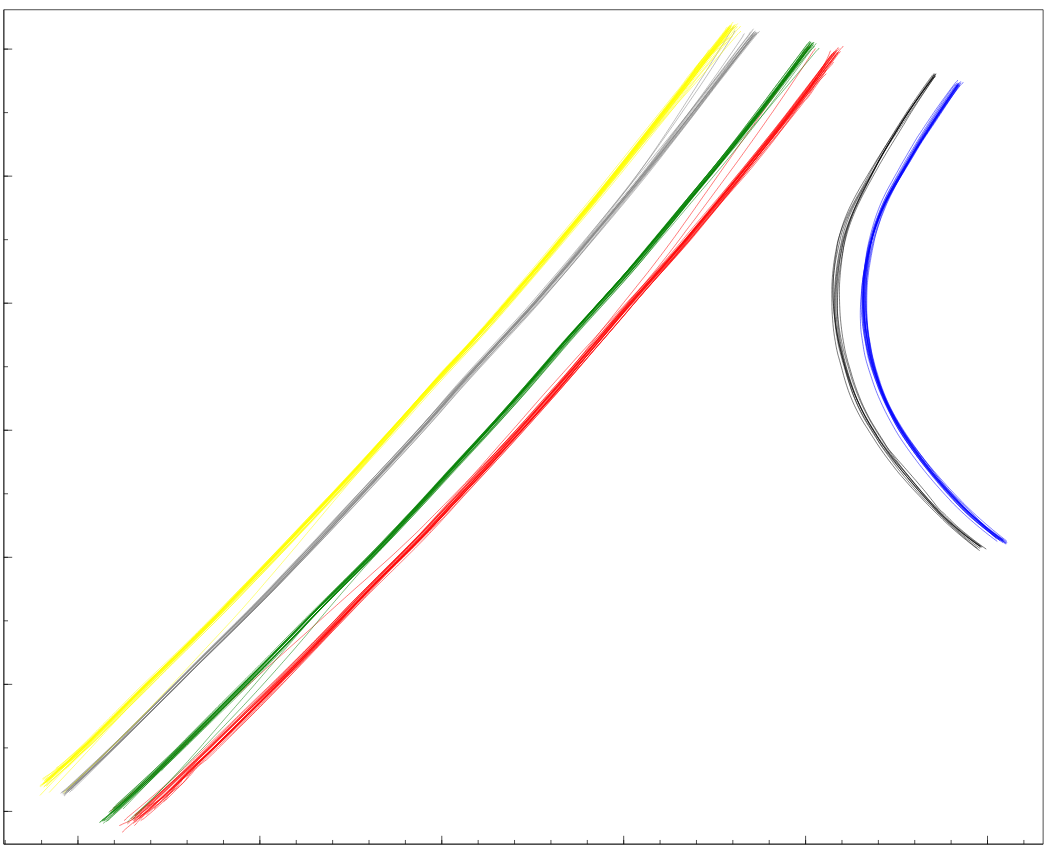
\includegraphics[align=c, width=0.4\linewidth]{resources/img/umsetzung/U1/dbscan_lcss/entennest}
    }}
    \qquad \qquad
    \subfloat[Datensatz Neckartor]{{
        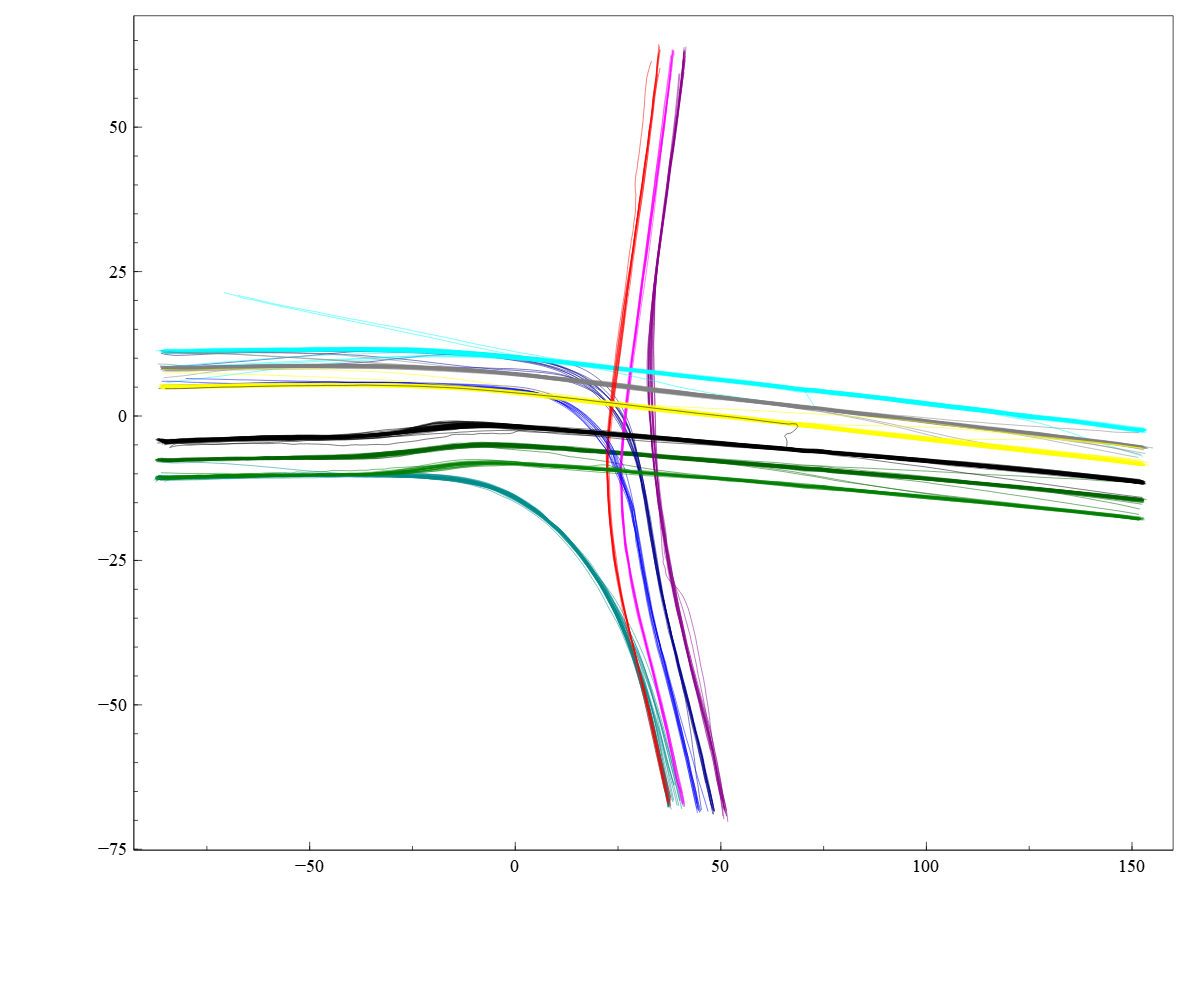
\includegraphics[align=c, width=0.4\linewidth]{resources/img/umsetzung/U1/dbscan_lcss/neckartor}
    }}
    \caption[Ergebnisse Clusteranalyse Ansatz DBSCAN und LCSS-Distanz]
            {Ergebnisse Clusteranalyse Ansatz DBSCAN und LCSS-Distanz - korrekte Unterteilung der Trajektorien in Spur-Cluster in a) und b)}
    \label{fig:real_results_dbscan_lcss}
\end{figure}

Der DBSCAN Algorithmus markiert atypische Trajektorien als Ausreißer, was den Vorteil hat, dass
diese nichtmehr anderen Spurclustern zugeordnet werden. Problematisch ist allerdings, dass Bewegungsbahnen
welche Abbiegevorgänge beschreiben und in unterschiedliche Spuren einbiegen, teilweise auch als Ausreißer
klassifiziert werden. In Abbildung \ref{fig:real_results_dbscan_lcss} b) fehlen so beispielsweise die Trajektorien
der zwei Abbiegespuren im oberen linken und unteren rechten Bereich (vergleiche Abbildung \ref{fig:real_neckartor} a)).
Um diese weiterhin erkennen zu können, wurde ein extra Verarbeitungsschritt eingeführt, welcher in Abschnitt
\ref{sec:real_detect_turning_lane} beschrieben wird.

Grundsätzlich überzeugten die Ergebnisse der Clusteranalyse. Die nachfolgend beschriebenen Schritte
der Spurerkennung basieren daher auf den Ergebnissen der hier vorgestellten Clustering-Methode.

\subsection{Erkennung von Abbiegespuren}
\label{sec:real_detect_turning_lane}

In Abschnitt \ref{sec:results_clustering_dbscan_lcss} wurde bereits erwähnt, dass, unter Verwendung des
gewählten Clustering-Verfahrens, einige Bewegungsbahnen als Ausreißer klassifiziert werden, dies eigentlich jedoch
nicht sind. Diese fälschlicherweise aussortierten Trajektorien beschreiben für gewöhnlich Abbiegevorgänge.
Problematisch an diesen Trajektorien ist, aus Sicht der Clusteranalyse, dass sie üblicherweise auf einer
gemeinsamen Spur -- der Abbiegespur -- beginnen, sich dann jedoch aufteilen und auf mehrere Fahrspuren verteilen.
Die Trajektorien haben aus diesem Grund, trotz anfänglich identischem Verlauf, zu hohe Distanzen zueinander, um
als ein Cluster identifiziert zu werden. Hinzu kommt, dass die Anzahl der Fahrzeuge, welche eine Abbiegespur
benutzen, häufig nicht hoch genug ist, damit auf Basis einer Abbiege-Variante ein Cluster geformt werden kann.
In Abbildung \ref{fig:real_turning_lane} a) und b) sind beispielhaft eine Abbiegespur der Neckartor-Kreuzung und
die dazugehörigen Trajektorien abgebildet. Anhand der Straßentopologie und der Trajektorien wird deutlich,
dass sich die Fahrzeuge nach dem Abbiegen auf drei Fahrstreifen verteilen.

\begin{figure}[H]
    \centering
    \subfloat[]{{
        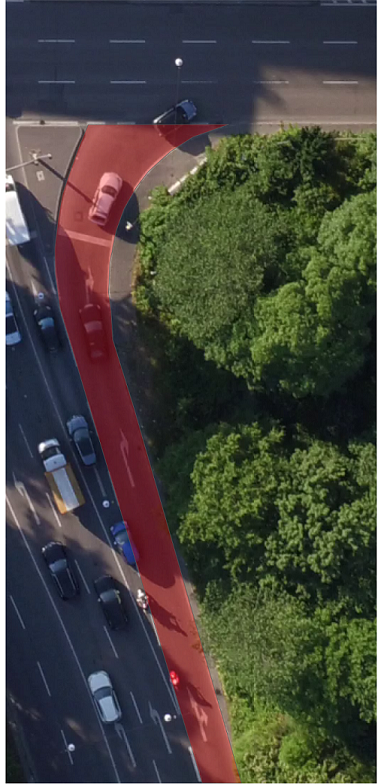
\includegraphics[align=c, width=0.14\linewidth]{resources/img/umsetzung/U1/turning_lane}
    }}
    \qquad \qquad \qquad
    \subfloat[]{{
        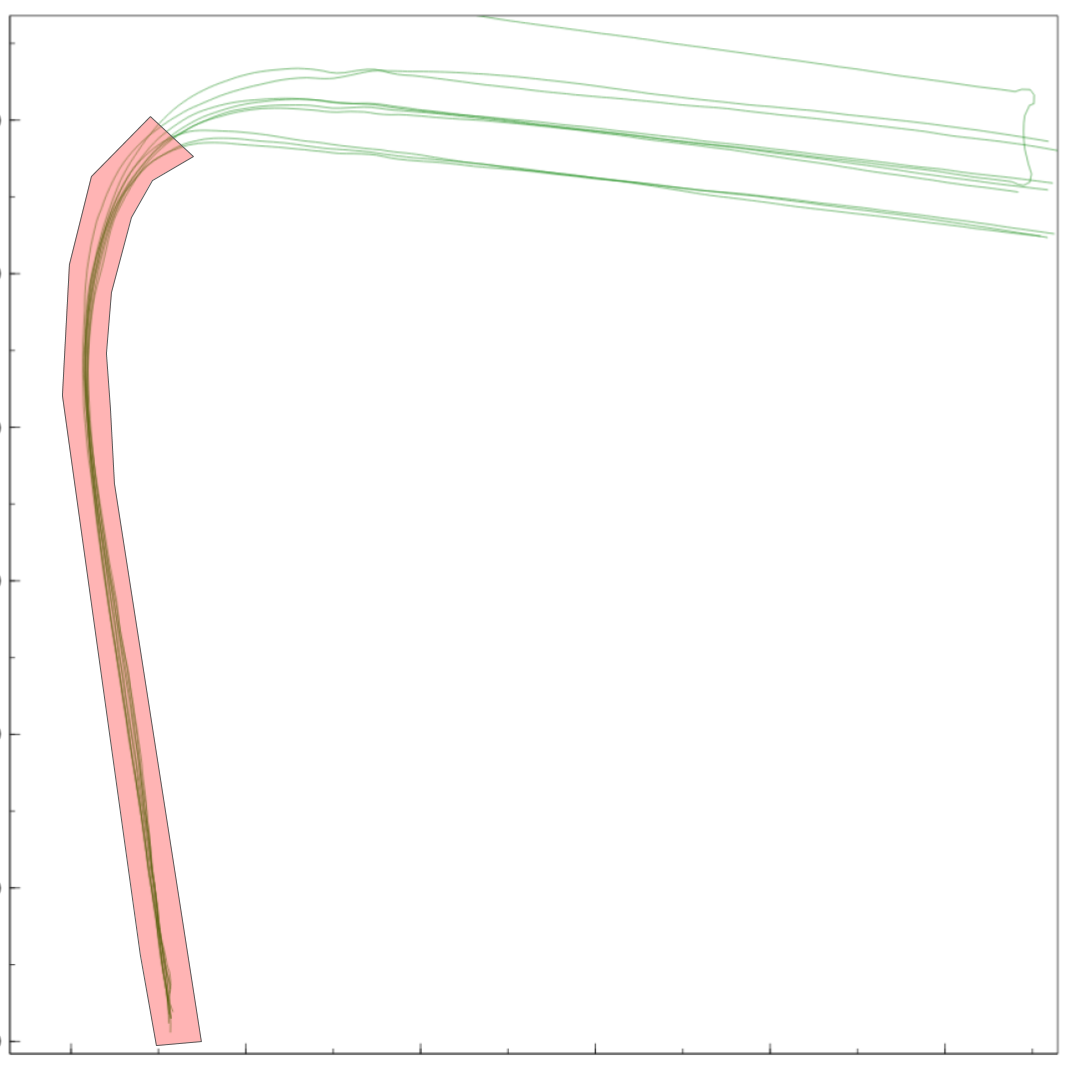
\includegraphics[align=c, width=0.28\linewidth]{resources/img/umsetzung/U1/turning_lane_trajs}
    }}
    \caption[Abbiegespur Neckartor Kreuzung]{Abbiegespur der Neckartor-Kreuzung a), zugehörige Trajektorien b)}
    \label{fig:real_turning_lane}
\end{figure}

Ziel des nachfolgend beschriebenen Verarbeitungsschrittes ist es, Trajektorien, welche Abbiegevorgänge
beschreiben, zu entsprechenden Clustern zusammenzufassen. Anhand dieser kann anschließend die Geometrie
der Spuren, wie für alle anderen Fahrspuren auch, bestimmt werden.
Die Cluster sollen hierbei allerdings nicht aus den kompletten Trajektorien gebildet werden, sondern
lediglich aus den Teilen, welche anfänglich identisch verlaufen. Dies ist konzeptionell in Abbildung
\ref{fig:real_turning_lane} b) dargestellt. Notwendig ist dies, da die Trajektorien nach dem Auseinanderlaufen
sehr unterschiedliche Bahnen beschreiben und daher keine eindeutigen Spur-Geometrien bestimmt werden können.

Um die oben beschriebenen Spurcluster zu finden, werden ausschließlich die Trajektorien untersucht,
welche während der Clusteranalyse als Ausreißer markiert wurden.
In einem ersten Schritt wird nach möglichen Trajektorie-Nachbarschaften gesucht. Hierzu wird für
jede Trajektorie $t$ der Abstand zwischen deren Start und allen anderen Trajektorie-Starts bestimmt.
Liegen mehr als fünf Trajektorie-Anfänge in einem Radius $laneEps = 1.5m$ um den Start von $t$, so bilden
die Trajektorien eine Nachbarschaft.
Dass die so gefunden Trajektorien auch tatsächlich den Verlauf einer Abbiegespur beschreiben und nicht
direkt auseinader laufen, wird anschließend geprüft.

Für eine Trajektorie-Nachbarschaft $N$ wird zunächst eine Referenz Bewegungsbahn $refT$ bestimmt, welche den
minimalen mittleren Abstand zu allen anderen Trajektorien besitzt:

\begin{ceqn}
\begin{align}
    refT_N = N(arg\ \underset{t\ \in\ N}{min}\ \Big(\frac{1}{|N|} \sum_{tt\ \in\ \{N \backslash t\}} D_{LCSS}(t, tt) \Big))
\end{align}
\end{ceqn}

Die Referenztrajektorie beschreibt die Nachbarschaft. Im Fall der Trajektorien aus Abbildung
\ref{fig:real_turning_lane} b) ist es beispielsweise eine Bahn, welche auf die mittlere Fahrspur abbiegt.
Nachdem $refT$ bestimmt wurde, wird die Trajektorie punktweise durchwandert. Es werden die Bereiche um jeden
Punkt überprüft, um so festzustellen, wo die Trajektorien der Nachbarschaft auseinanderlaufen. Der hierzu
eingesetzte Algorithmus ist in Listing \ref{lst:pseudo_split_point} vereinfacht beschrieben.
\begin{lstlisting}[caption=Pseudocode Split-Punkt Bestimmung, language=Pseudo, label=lst:pseudo_split_point]
algorithm findSplitPoint:
  input:  neighborhood: N, reference-trajectory: refT
  output: point where trajectories of neighborhood split up

  for each point in refT do
    regionAroundP := create circular region around point with r = laneEps
    neighborsInReg := count intersections of trajectories with regionAroundP

    if neighborsInReg <= 0.75 * |N| && idx(point) > 0.33 * refT.pointLength then
      return point
    end
  end

  return None
\end{lstlisting}

Zur Bestimmung der Regionen um einen Punkt und der Schnittpunkte der Trajektorien mit diesem Bereich,
wird die JTS Topology Suite\footnote{JTS Topology Suite: \url{https://locationtech.github.io/jts/}}
(JTS) eingesetzt. Der Split-Punkt einer Nachbarschaft ist jener Punkt, in dessen Umfeld die Anzahl der
Trajektorien erstmals unter 75\% fällt. Er ist zudem nur gültig, wenn er nicht im ersten Drittel der
Referenztrajektorien liegt.

Nachdem der Split-Punkt einer Nachbarschaft gefunden wurde, werden alle in ihr beinhalteten Bewegungsbahnen
an jenem Trajektorie-Punkt geteilt, der dem Split-Punkt am nächsten ist.
Die so neu erstellten Trajektorien bilden ein neues Cluster. In Abbildung \ref{fig:real_turning_lane_result}
sind alle Spurcluster dargestellt, welche nach diesem Schritt existieren. Die zwei Cluster der Abbiegespuren,
welche in Abbildung \ref{fig:real_results_dbscan_lcss} b) noch fehlten, sind nun auch vorhanden.

\begin{figure}[H]
    \centering
    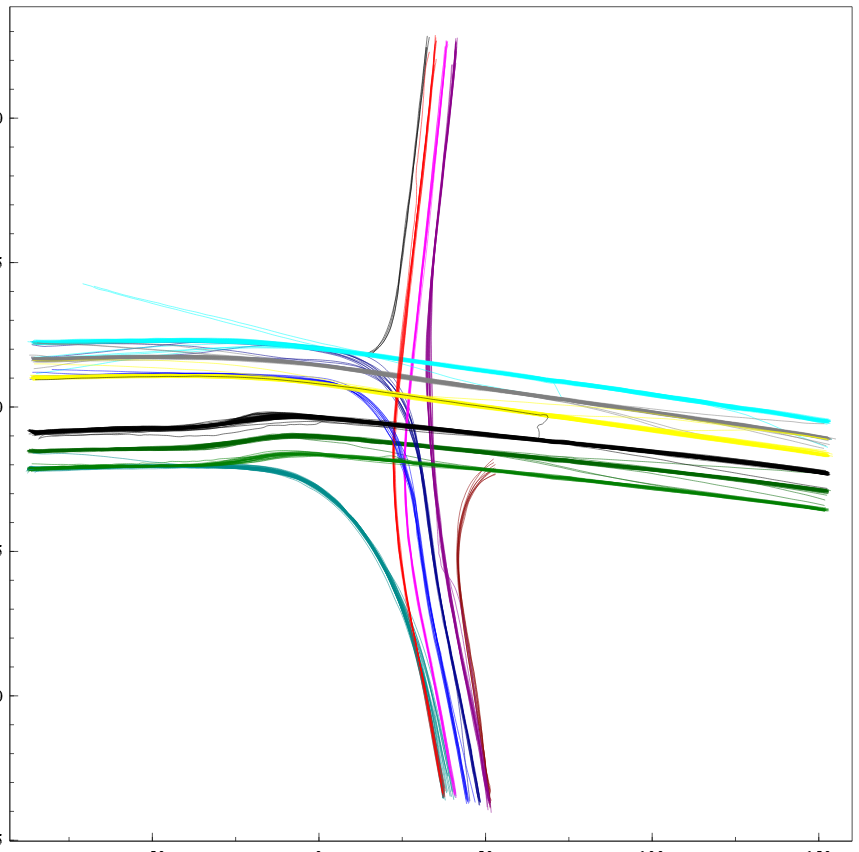
\includegraphics[width=0.35\linewidth]{resources/img/umsetzung/U1/clusters_with_turning_lanes}
    \caption{Ergebnis Clusteranalyse inklusive Abbiegespur-Cluster}
    \label{fig:real_turning_lane_result}
\end{figure}

Mithilfe der oben vorgestellten Verfahren können Trajektorie-Cluster entdeckt werden, welche
die einzelnen Fahrspuren in einer Aufnahme beschreiben. Im nachfolgenden Abschnitt wird noch ein
zusätzliches Verfahren vorgestellt, mit dessen Hilfe sich die Clusteranalyse automatisch parametrisieren lässt.

\subsection{Automatische Parametrisierung der Clusteranalyse}
\label{sec:real1_adjustment_clustering_parameter}

Das oben beschriebene Clustering-Verfahren erkennt, unter Verwendung der in Abschnitt \ref{sec:results_clustering_dbscan_lcss}
definierten Standardparameter, Spur-Cluster in den meisten Trajektoriedatensätzen zuverlässig.
Das Verfahren mit Standardparametrisierung stößt allerdings an seine Grenzen, wenn sich die Trajektorien unterschiedlicher Fahrspuren
in einem Datensatz über eine größere Strecke hinweg stark überlagern. Dies ist beispielsweise im Datensatz
\textit{Düsseldorf} der Fall, dessen Trajektorien in Abbildung \ref{fig:real1_clusters_duesseldorf} a) dargestellt sind.
Es ist erkennbar, dass die zwei oben liegenden Fahrspuren sich nach circa 400 Metern auf vier Fahrspuren aufteilen.
Herausfordernd für die Clusteranalyse ist zudem, dass der Datensatz sehr viele Bewegungsbahnen beinhaltet,
welche Spurwechselvorgänge beschreiben.
Das Ergebnis der Clusteranalyse unter Verwendung der Standardparameter für den \textit{Düsseldorf} Datensatz ist
in Abbildung \ref{fig:real1_clusters_duesseldorf} b) dargestellt.

\begin{figure}[H]
    \centering
    \subfloat[]{{
        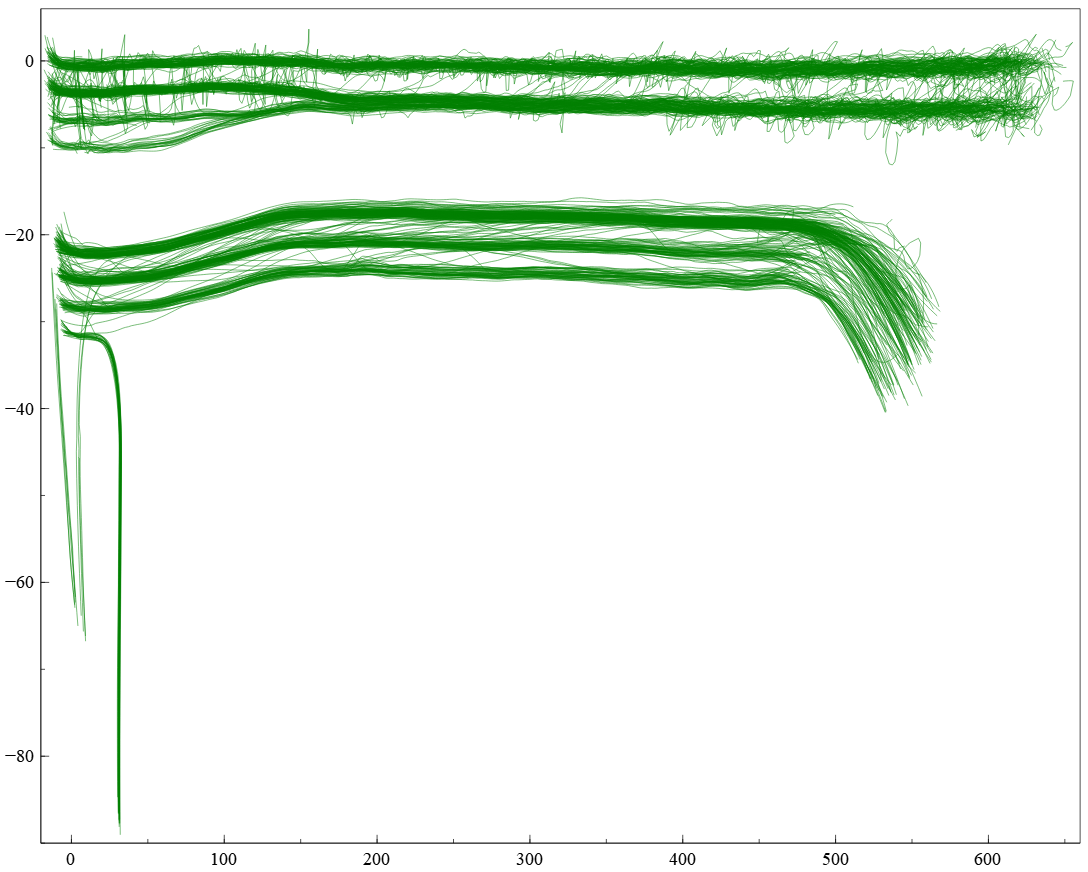
\includegraphics[align=c, width=0.33\linewidth]{resources/img/umsetzung/U1/Plots_Duesseldorf/preProTraj}
    }}
    \subfloat[]{{
        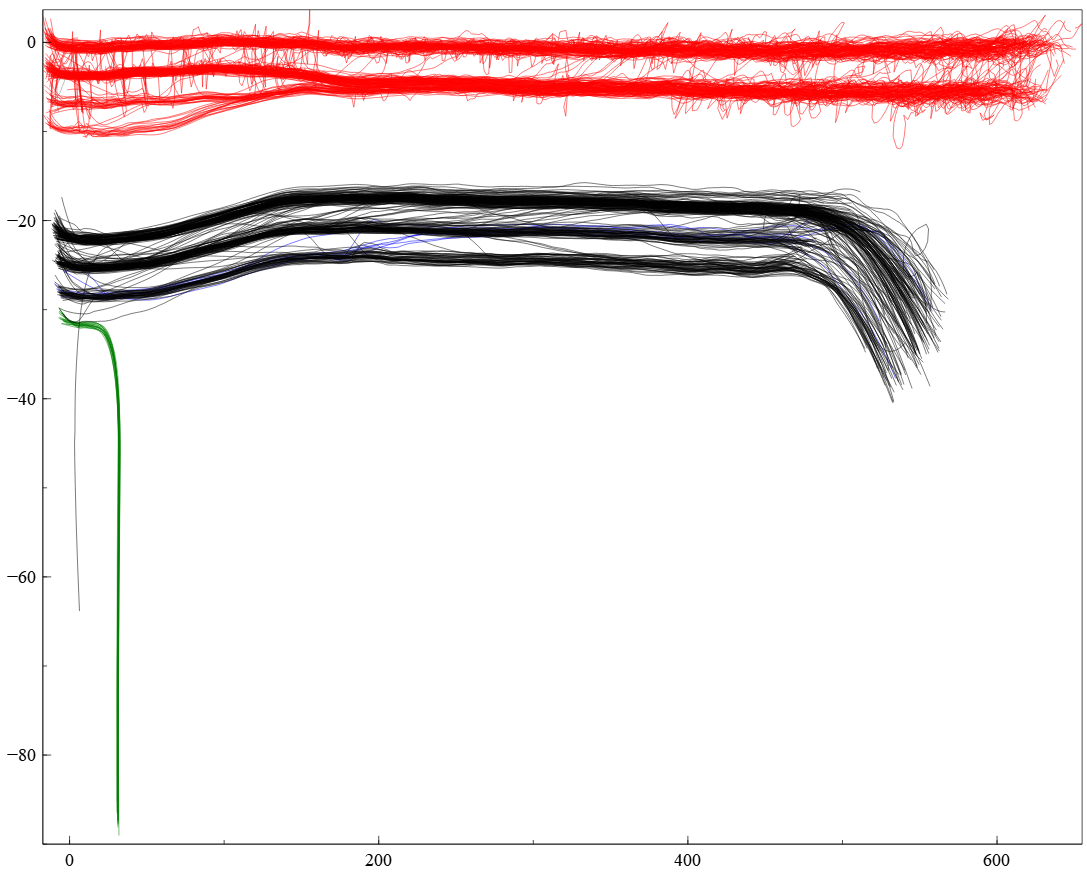
\includegraphics[align=c, width=0.33\linewidth]{resources/img/umsetzung/U1/Plots_Duesseldorf/filteredClusters_03}
    }}
    \subfloat[]{{
        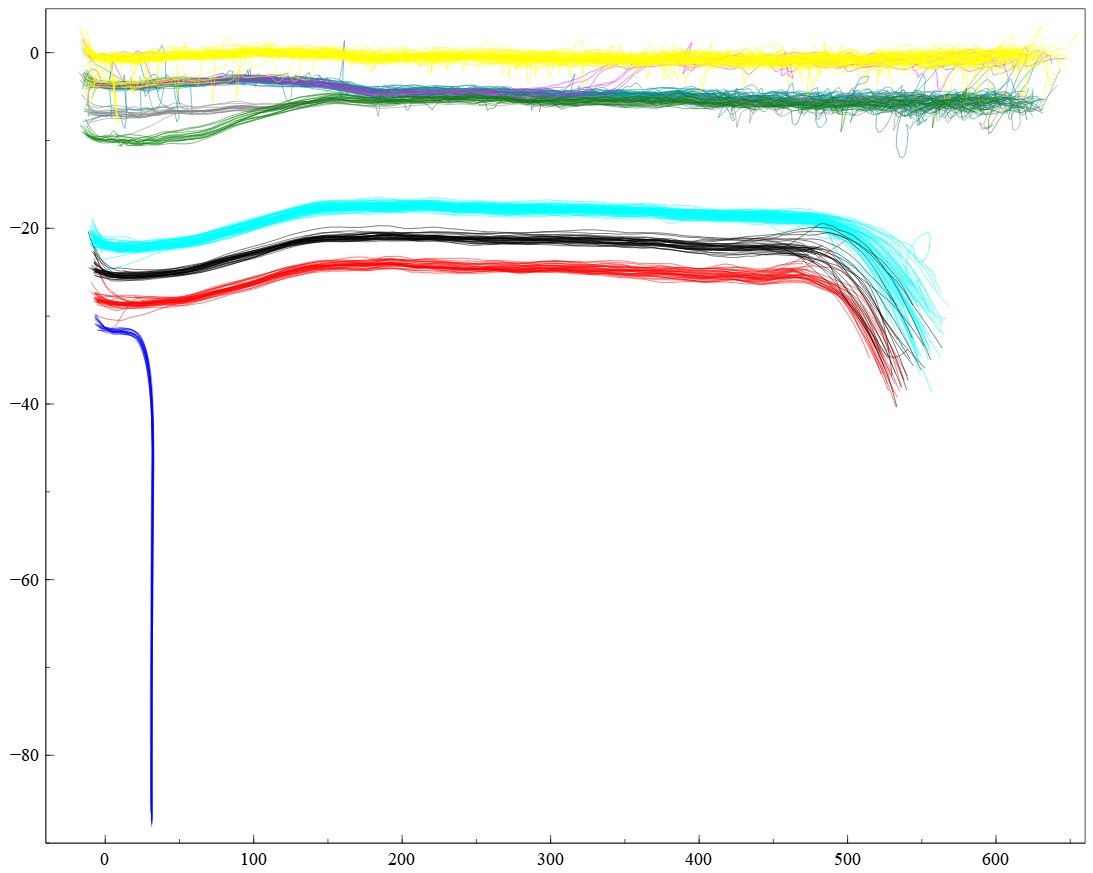
\includegraphics[align=c, width=0.33\linewidth]{resources/img/umsetzung/U1/Plots_Duesseldorf/filteredClusters}
    }}
    \caption[Ergebnis Clusteranalyse Düsseldorf Datensatz]
            {a) Roh-Trajektorien des Datensatzes Düsseldorf, b) Ergebnis der Clusteranalyse unter Verwendung
            der Standardparameter ($\epsilon_{DBSCAN} = 0.3$), c) Erwünschtes Clustering-Ergebnis unter Verwendung $\epsilon_{DBSCAN} = 0.1$}
    \label{fig:real1_clusters_duesseldorf}
\end{figure}

Es ist erkennbar, dass das Clustering-Verfahren die einzelnen Fahrspuren nicht korrekt identifizieren
kann. Das gewünschte Ergebnis wird allerdings erzielt, wenn der Standardwert für den Parameter $\epsilon_{DBSCAN}$
von $0.3$ auf $0.1$ reduziert wird. Um das Verhalten der Clusteranalyse in dieser Hinsicht steuern zu können,
wurde dem Nutzer die Möglichkeit gegeben, $\epsilon_{DBSCAN}$ beim Start der Spurerkennung anzupassen.
Da das manuelle Setzen des Wertes allerdings Expertenwissen voraussetzt, wurde zudem ein Verfahren entwickelt,
welches $\epsilon_{DBSCAN}$ automatisch anpasst, wenn die identifizierten Spur-Cluster beziehungsweise Fahrspuren
nicht mit den realen Spuren übereinstimmen.

Das Verfahren nutzt die Spur-Geometrien, welche auf Basis
der identifizierten Spur-Cluster ermittelt werden (siehe Abschnitt \ref{cha:lane_definition}).
Mithilfe der Geometrien, welche sich jeweils aus einem Trajektorie-Cluster ableiten, und den Trajektorien des
Clusters, lassen sich sogenannte \textit{Weg-Zeit-Diagramme} erstellen, welche die Bewegungen der Fahrzeuge auf einer
Fahrspur abbilden.
Beschreibt eine ermittelte Spur-Geometrie eine reale Fahrspur korrekt, dann schneiden sich die Trajektorien
in dem entsprechenden Weg-Zeit-Diagramm nicht, da die Fahrzeuge auf der Spur hintereinander herfahren
und sich nicht überholen können. Ein entsprechendes Diagramm ist in Abbildung \ref{fig:real1_way_time_diagramms} a) zu sehen.
Beschreibt eine Spur-Geometrie hingegen, aufgrund einer fehlerhaften Clusteranalyse, mehrere reale Fahrspuren
und ist daher zu breit, dann existieren in dem dafür erstellten Weg-Zeit-Diagramm Überschneidungen von Trajektorien,
da die Fahrzeuge sich auf den realen Fahrspuren überholen können. Ein solches Diagramm ist in
Abbildung \ref{fig:real1_way_time_diagramms} b) dargestellt.

\begin{figure}[H]
    \centering
    \subfloat[]{{
        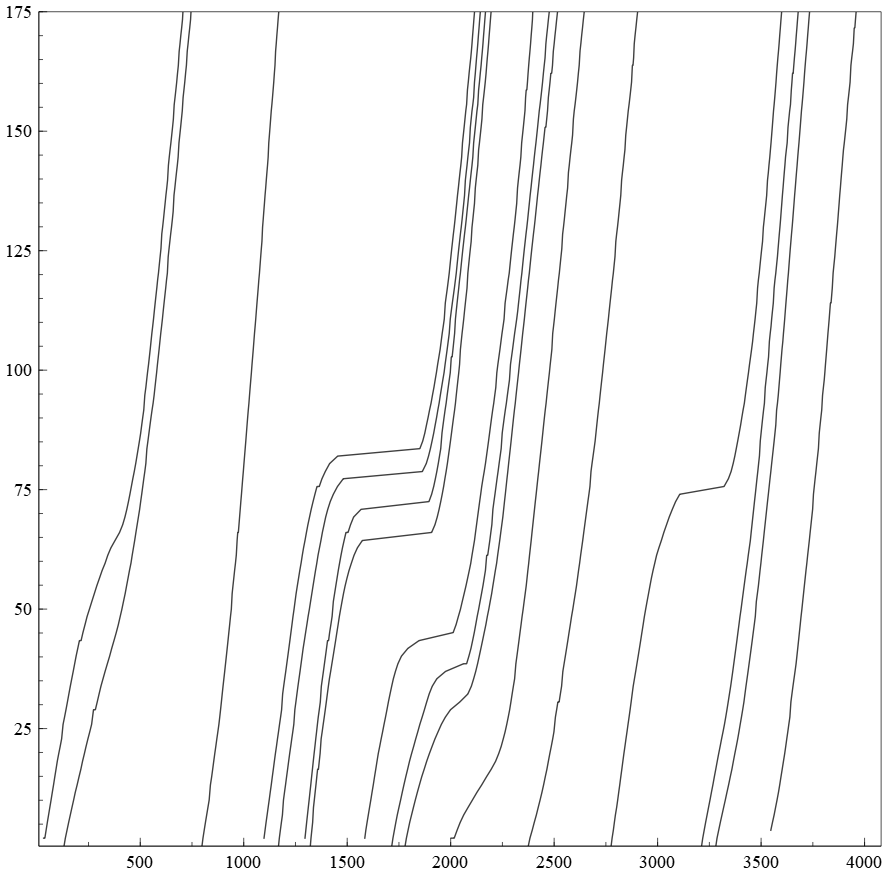
\includegraphics[align=c, width=0.35\linewidth]{resources/img/umsetzung/U1/way_time_lines_without_crossings}
    }}
    \qquad
    \subfloat[]{{
        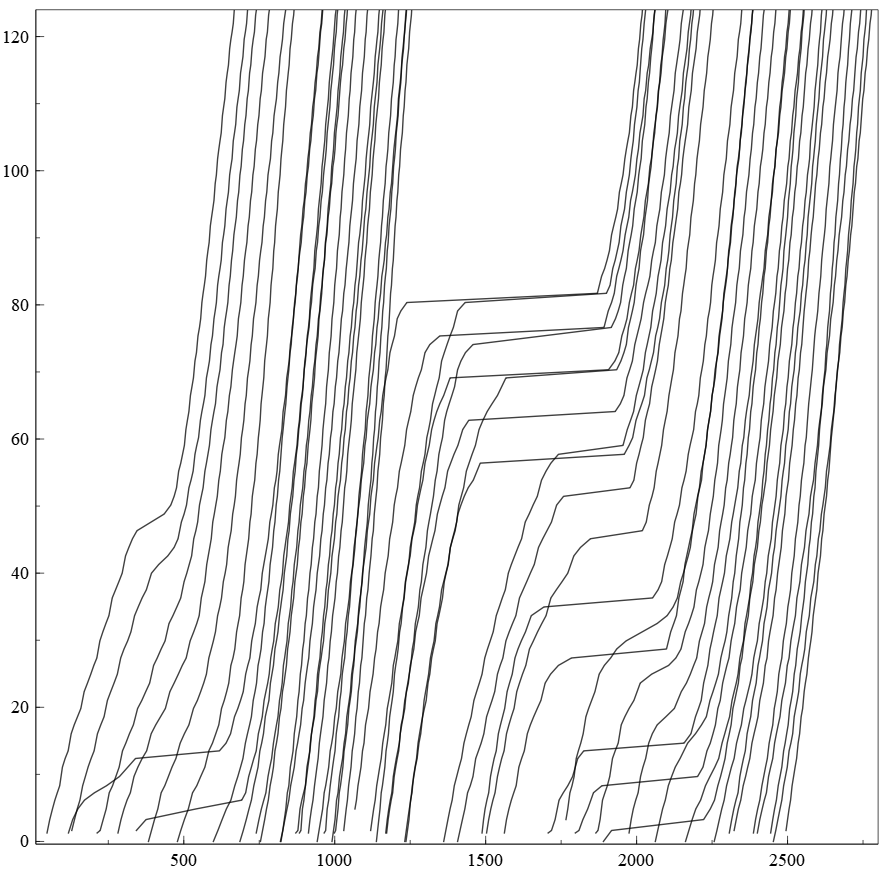
\includegraphics[align=c, width=0.35\linewidth]{resources/img/umsetzung/U1/way_time_lines_with_crossings}
    }}
    \caption[Weg-Zeit-Diagramme mit und ohne Trajektorie-Schnittpunkten]
            {a) Weg-Zeit-Diagramm ohne Trajektorie-Überschneidungen, b) Weg-Zeit-Diagramm mit Trajektorie-Überschneidungen}
    \label{fig:real1_way_time_diagramms}
\end{figure}

Der Algorithmus zur Anpassung des Clustering-Parameters $\epsilon_{DBSCAN}$ nutzt die oben beschriebene
Eigenschaft der Weg-Zeit-Diagramme, um zu erkennen, ob die ermittelten Spur-Geometrien mit den realen
Fahrspuren übereinstimmen, oder ob diese weiter untergliedert werden müssen.
Der Ablauf des Verfahrens kann grob wie folgt beschrieben werden:

\begin{enumerate}
    \item Durchführung der Spurerkennung.
    \item Erstellung von Weg-Zeit-Trajektorien auf Basis der Spur-Geometrien.
    \item Bestimmung der Anzahl der Überschneidungen in den Weg-Zeit-Trajektorien:
    \begin{enumerate}
        \item bei Überschreitung des Grenzwertes $\rho$: Zurück zu 1) und Anpassung von\\ $\epsilon_{DBSCAN}$, sonst
        \item Verwendung der ermittelten Spur-Geometrien.
    \end{enumerate}
\end{enumerate}

Der Wert für $\epsilon_{DBSCAN}$ wird in diesem iterativen Verfahren nicht sukzessive reduziert oder erhöht,
sondern es werden verschiedene, vordefinierte Werte getestet, welche in unterschiedlichen Situationen
gute Ergebnisse liefern.
Unter Verwendung des Verfahrens werden beispielsweise auch im Fall des \textit{Düsseldorf} Datensatzes die erwarteten
Spur-Cluster identifiziert, welche in Abbildung \ref{fig:real1_clusters_duesseldorf} c) zu sehen sind.

Dank der Parameteranpassung kann das Verhalten der Clusteranalyse automatisch geändert werden,
wenn die Ergebnisse nicht die erwartete Qualität besitzen. Dem Nutzer wird dadurch eine eventuell notwendige
manuelle Parametrisierung abgenommen.